% !TeX spellcheck = es_ES
\chapter{Estado del arte }\label{chapter:review}

% \begin{itemize}
% 	\item Realizar una introducción sobre el contenido 
% 	\item Hablar un poco de la estructura del capítulo.
% 	 \item En la sección de Meta-Learning se define el problema de meta-learning, se dan definiciones del mismo y se realiza un estudio de meta-learning aplicado al problema de la selección de modelos separados por el tipo de solución que se da para el mismo ~\ref{sec:metalearning}
% 	\item La sección de AutoML se define el problema de AutoML, se da una (o varias) definiciones del concepto de AutoML y se realiza un estudio del mismo desde los diferentes tipos de métodos de optimización usados para la selección de modelos, destacando el uso de meta-learning. ~\ref{sec:automl}
% \end{itemize}
 
Este capítulo proporciona una introducción a los campos y los trabajos que están relacionados con las técnicas utilizadas en esta tesis. Se comienza introduciendo las ideas básicas de meta-learning (Sección \ref{sec:metalearning}), definiendo el problema que este campo resuelve, explicando la estructura de un sistema de meta-learning y varias de sus aplicaciones. El objetivo fundamental de este trabajo es añadir componentes de meta-learning a un sistema de \textit{Automated Machine Learning} (AutoML), así que este campo es introducido (Sección \ref{sec:automl}). Se presentan diferentes formulaciones teóricas del problema de AutoML y se describen los componentes fundamentales de un proceso de AutoML, así como ejemplos de sistemas para cada uno de los enfoques existentes. El área de interés de esta investigación es la aplicación de meta-learning para la selección de modelos, en concreto, su utilización para añadir conocimiento en sistemas AutoML, por lo que varias técnicas para la solución de este problema son estudiadas (Sección \ref{sec:metalearning-automl}).

\section{Meta-Learning}\label{sec:metalearning}

%\begin{itemize}
%	\item[$\checkmark$] Introducir esta sección hablando un poco del concepto de meta-learning y un poco de su historia (referirse a los papers: \textit{Metalearning: A survey of trends and technologies} y \textit{A Comprehensive Overview and Survey of Recent Advances in Meta-Learning})
%\end{itemize}

El término meta-learning ocurrió por primera vez en el área de psicología educacional. Uno de los investigadores más citados en este campo, John Biggs, describió meta-learning ``como ser consciente y tomar el control del conocimiento de uno''~\cite{biggs1985role}. Por lo tanto, meta-learning es visto como un entendimiento y adaptación del aprendizaje en sí en un nivel más alto que simplemente adquirir conocimiento de una materia. Una persona consciente y capaz de meta-learning es capaz de evaluar su enfoque de aprendizaje de acuerdo a los requerimientos de una tarea en específico.

Meta-learning usada en el contexto de aprendizaje automático tiene muchas similitudes a esta descripción. El conocimiento de una materia se traduce en \textit{base-learning}, donde la experiencia es acumulada para una tarea en específico. Meta-learning empieza en un nivel mayor y se encarga de acumular experiencia sobre varias aplicaciones de un sistema de aprendizaje~\cite{hospedales2021metalearning}.

Debido al creciente poder de computación y gran disponibilidad de conjuntos de datos en los últimos 20 años, la investigación de aprendizaje automático enfrentó un creciente número de algoritmos disponibles, incluyendo multitudes de parametrizaciones, enfoques de pre-procesamiento y post-procesamiento, así como una gran variedad de aplicaciones~\cite{lemke2013metalearning}. Promoviendo un mejor entendimiento del aprendizaje automático en sí, meta-learning puede ser de una ayuda invaluable, evitando procedimientos extensivos de prueba y error para la selección de algoritmos. Además, puede permitir entender mejor que hace a un determinado algoritmo desempeñarse bien en un determinado problema. En esta sección se estudia la definición de meta-learning, la estructura de un sistema de meta-learning y algunas de sus aplicaciones.

\subsection{Definición}\label{subsec:mtl-definition}

%\begin{itemize}
%	\item[$\checkmark$] Hablar de distintas definiciones formales del término de meta-learning (referirse a:  \textit{Metalearning: A survey of trends and technologies})
%\end{itemize}

La primera definición de meta-learning en el campo de aprendizaje automático fue dado por J\"ugen Schmidhuber en 1987, el cual lo considera la interacción entre agente y el ambiente impulsando la superación personal en el agente. Un gran conjunto de definiciones ha sido dada desde entonces, la siguiente lista fue obtenida de Lemke et al~\cite{lemke2013metalearning}:

\begin{enumerate}
	\item Meta-learning estudia como los sistemas de aprendizaje puede incrementar en eficiencia a través de la experiencia; el objetivo es entender cómo el aprendizaje en sí puede hacerse flexible de acuerdo al dominio o la tarea sujeto de estudio~\cite{vilalta2001perspective}.
	\item El principal objetivo de meta-learning es entender la interacción entre el mecanismo de aprendizaje y los contextos concretos en los cuales ese mecanismo es aplicable~\cite{giraud2008metalearning}.
	\item Meta-learning es el estudio de los métodos principales que explotan el meta-conocimiento para obtener modelos eficientes y soluciones adaptando los procesos de aprendizaje automático y minería de datos~\cite{bradzil2009metalearning}.
	\item Meta-learning monitorea el proceso de aprendizaje automático en sí, en el contexto de aprender los problemas que encuentra, e intenta adaptar su comportamiento para desempeñarse mejor~\cite{vanschoren2010understanding}.
\end{enumerate}

En la mayoría de las definiciones son conceptos claves sistemas de aprendizaje que se adaptan y mejoran con la experiencia, excepto en la definición 2. Esta enfatiza en una mejor comprensión de la interacción entre dominios y mecanismos de aprendizaje, lo cual no necesariamente implica el objetivo de un sistema de aprendizaje mejorado, sino la búsqueda de un mejor entendimiento de cuáles tareas tienen éxito o fallan.

Meta-learning es mejor entendido comúnmente como ``aprendiendo a aprender'', lo cual se refiere al proceso de mejorar un algoritmo de aprendizaje a través de múltiples episodios de aprendizaje. En contraste, el aprendizaje automático convencional mejora las predicciones del modelo sobre múltiples instancias de datos. Durante el \textit{base-learning} o aprendizaje base, un algoritmo de aprendizaje interior (o inferior/base) resuelve una tarea como clasificación de imágenes, definida por un dataset y un objetivo. Durante \emph{meta-learning}, un algoritmo externo (o superior/meta) actualiza el algoritmo interior de tal manera que el modelo que aprende mejora un objetivo externo. Los episodios de aprendizaje de la tarea base pueden ser vistos como una forma de proveer las instancias necesitadas por el algoritmo externo para aprender el algoritmo de aprendizaje base~\cite{hospedales2021metalearning}. 

Meta-learning difiere de \textit{base-learning} en el alcance del nivel de adaptación. Mientras que el aprendizaje en un nivel base está enfocado en acumular experiencia en una tarea específica, el aprendizaje en meta-learning tiene el objetivo de acumular experiencia en el rendimiento de múltiples aplicaciones de un sistema de aprendizaje. De esta forma, muchos algoritmos convencionales tales como la búsqueda aleatoria de hiperparámetros mediante validación cruzada podrían caer en la definición de meta-learning. La característica destacada del \emph{meta-learning} contemporáneo es un meta-objetivo explícitamente definido, y una optimización de extremo a extremo del algoritmo interior con respecto a este objetivo.

\subsection{Campos relacionados}\label{subsec:mtl_related_fields}

%\begin{itemize}
%	\item[$\checkmark$] Mencionar y resumir algunas áreas relacionadas con meta-learning, para incluir AutoML (referirse a: \textit{Meta-Learning in Neural Networks: A Survey})
%	\item No estoy segura si esta sección es necesaria...
%\end{itemize}

Aquí posicionamos meta-learning contra áreas relacionadas cuya relación con meta-learning es a menudo una fuente de confusión \cite{hospedales2021metalearning}:

\begin{description}
	\item[Transfer Learning (TL):] TL usa experiencia pasada de una tarea fuente para mejorar el aprendizaje (la velocidad, la eficiencia de los datos, la precisión) de una tarea destino. TL se refiere a esta área de problemas como familia de soluciones, y para su solución hace uso de la transferencia de parámetros, más el ajuste opcional de los mismos. En contraste, meta-learning se refiere al paradigma que puede ser utilizado para mejorar TL, así como otros problemas. En TL el modelo final es extraído por aprendizaje simple en la tarea fuente sin el uso de un meta-objetivo. En meta-learning, el modelo final estaría definido por la optimización externa que evalúa el beneficio del modelo cuando aprende una nueva tarea. % De una forma más general, \emph{meta-learning} trata con un rango mucho más grande de meta-representaciones.
	
	\item[Aprendizaje multi-tarea (MTL):] intenta aprender en conjunto algunas tareas relacionadas para beneficiarse de la regularización debido al intercambio de parámetros y la diversidad de la representación compartida resultante. Como TL, MTL convencional es una optimización de un solo nivel sin un meta-objetivo. Además, el propósito de MTL es el de aprender de una cantidad fija de tareas conocidas, mientras que el objetivo de meta-learning es a menudo aprender de tareas futuras no vistas.
	 
	\item[Optimización de Hiperparámetros (HPO):] está dentro de las consideraciones de meta-learning, en el sentido de que hiperparámetros como la tasa de aprendizaje o la fuerza de regularización describen ``cómo aprender''. Aquí se suelen incluir tareas de HPO que definen un meta-objetivo que es entrenado de extremo a extremo con redes neuronales, tales como el aprendizaje de hiperparámetros basados en gradientes y la búsqueda de arquitectura neuronal. Pero excluyen otros enfoques como búsqueda aleatoria y optimización bayesiana, las cuales raramente están consideradas como meta-learning~\cite{hospedales2021metalearning}.
	
	\item[AutoML:] AutoML es más bien un espectro amplio de enfoques con el objetivo de automatizar partes del proceso de aprendizaje automático que son típicamente manuales, tales como la preparación de los datos, la selección de algoritmos, ajuste de hiperparámetros, y búsqueda de arquitecturas. AutoML a menudo utiliza numerosas heurísticas afuera del alcance de meta-learning, y se usa en tareas como limpieza de datos, que son menos importantes en meta-learning. Sin embargo, AutoML a veces utiliza optimizaciones de extremo a extremo de un meta-objetivo, así que meta-learning puede ser visto como una especialización de AutoML. AutoML a menudo usa técnicas de meta-learning para inicializar su proceso de optimización y ganar experiencia de experimentaciones pasadas, como se estudia en la Sección \ref{sec:metalearning-automl}.
\end{description}

\subsection{Estructura de un Sistema de Meta-Learning}

Un sistema de meta-learning está compuesto esencialmente por dos partes. Una parte tiene la tarea de adquirir meta-conocimiento de sistemas de aprendizaje automático. La otra parte tiene el objetivo de aplicar este meta-conocimiento a nuevos problemas con el objetivo de identificar un algoritmo o técnica de aprendizaje óptimo.

\subsubsection{Adquisición de Meta-Conocimiento} 

Hay dos modos naturales en los cuales el meta-conocimiento puede ser adquirido. Una posibilidad es depender de conocimiento experto y otra posibilidad es usar un procedimiento automático. 

La obtención de meta-conocimiento a través del conocimiento experto se realiza en la forma de reglas que coinciden con las características de dominio (dataset) y con algoritmos de aprendizaje automático. Estas reglas pueden ser hechas a mano, teniendo en cuenta resultados teóricos, el conocimiento humano y evidencia empírica. Sin embargo, este método tiene serias desventajas: el conjunto de reglas resultantes probablemente esté incompleto y el mantenimiento del conjunto de reglas a medida que nuevos algoritmos se vuelven disponibles es problemático. Como resultado, la mayoría de la investigación se ha enfocado en métodos automáticos~\cite{bradzil2017metalearning}.
	
Para la automatización de la adquisición de conocimiento es necesario un conjunto de problemas (datasets) y un conjunto de algoritmos de aprendizaje automático que queremos considerar. Entonces se necesita definir un método experimental que determine con cuáles alternativas deberíamos experimentar y en qué orden. Por ejemplo, dado un dataset (con ciertas características) y ciertos algoritmos de aprendizaje automático, se producen resultados de rendimiento para cada uno de estos algoritmos a través de un método de evaluación (como validación cruzada). Los resultados y la estructura de los algoritmos aplicados, junto con la caracterización de los datasets, representan un pedazo de información que es guardado en una base de meta-conocimiento. El proceso es entonces repetido para otras combinaciones de datasets y algoritmos. 
En la Figura~\ref{fig:adquisition} se muestra cómo se realiza el proceso de adquisición del meta-conocimiento. %Dado un conjunto de datasets se aplica un conjunto de algoritmos. Los resultados de rendimiento obtenidos en estos datasets y la estructura de los algoritmos son guardados junto con las meta-características de los datasets en la base de meta-conocimiento.

 \begin{figure}[H]
 	\centering
 	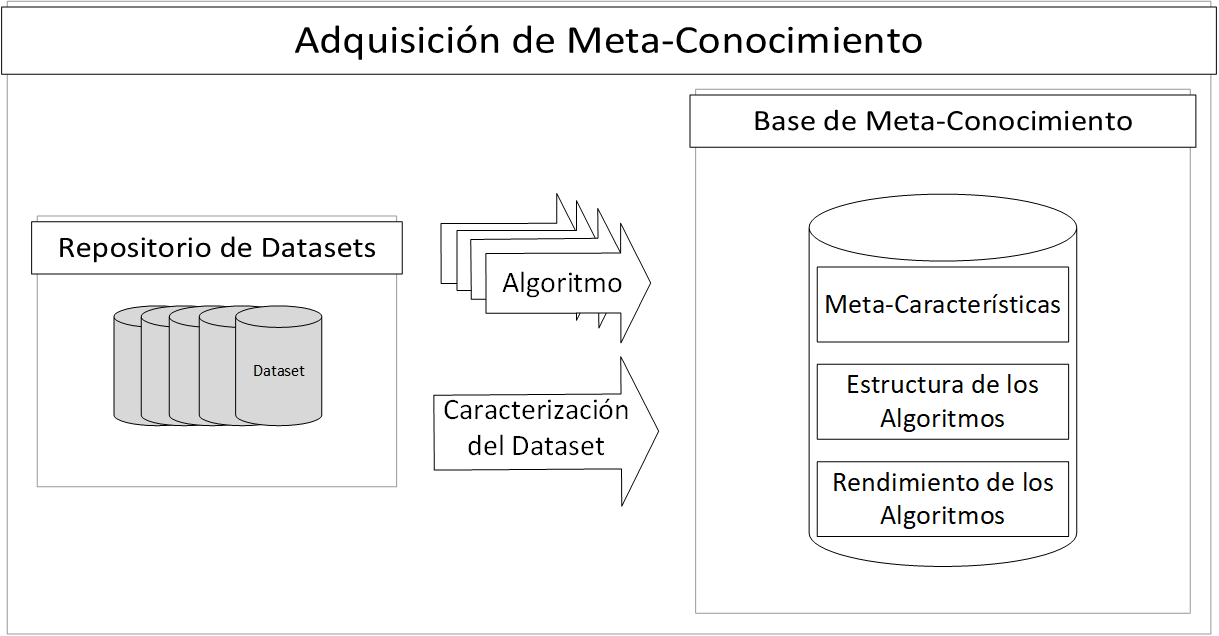
\includegraphics[scale=.5]{Figures/adquisition.png}
 	%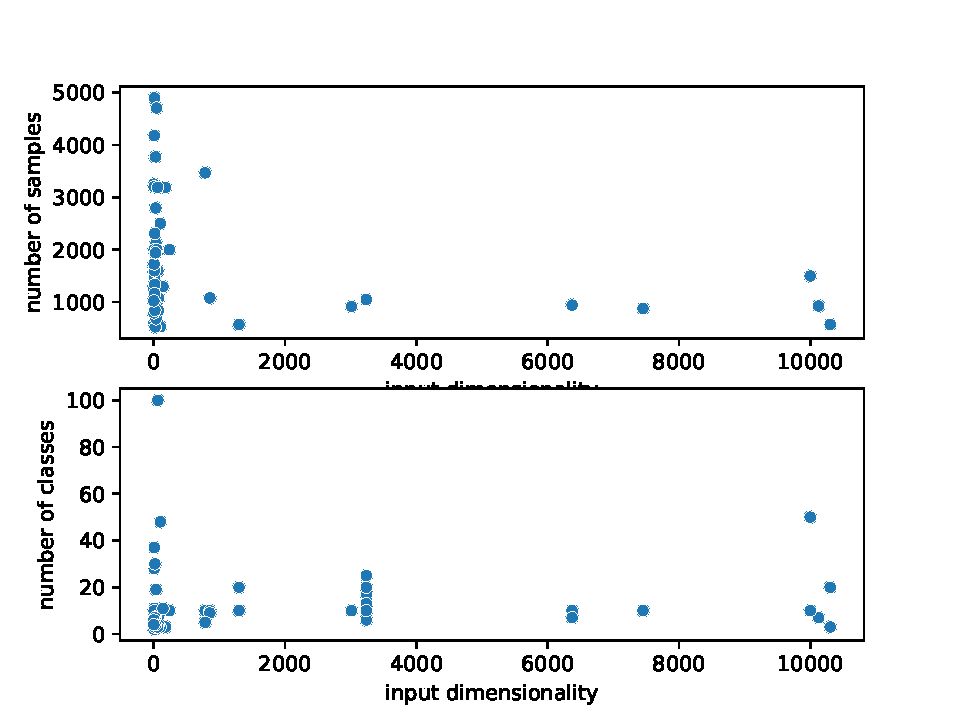
\includegraphics[scale=.60]{Figures/mtf scatterplot.pdf}
 	\caption{Proceso de adquisición de meta-conocimiento. }
 	\label{fig:adquisition}
 \end{figure}


\subsubsection{Aplicación de Meta-Conocimiento}

En un sistema de meta-learning la aplicación de meta-conocimiento puede ser usada para ayudar a seleccionar o adaptar algoritmos de aprendizaje automático. Por ejemplo, podemos considerar nuestro problema de la selección de algoritmos de aprendizaje automático dado un determinado conjunto de algoritmos. Este puede ser visto como un problema de búsqueda, donde el espacio de búsqueda incluye los algoritmos de aprendizaje automático individuales y el objetivo es identificar el mejor algoritmo. Este proceso puede ser dividido en dos fases separadas. La Figura~\ref{fig:application} muestra un diagrama de como ocurre este proceso.

En la primera fase (Figura~\ref{fig:application} a) el objetivo es identificar un subconjunto adecuado de algoritmos de aprendizaje automático basados en un dataset de entrada. El método de selección empleado en ese proceso se basa en el meta-conocimiento. Dado un nuevo dataset sus meta-características son extraídas y estas son analizadas para extraer de la base de meta-conocimiento los datasets similares. Por lo general, el resultado de esta fase es representado en la forma de un subconjunto rankeado de algoritmos de aprendizaje automático.

La segunda fase (Figura~\ref{fig:application} b) tiene el objetivo de buscar a través del espacio reducido. Cada opción es evaluada empleando una métrica de rendimiento determinado (por ejemplo, \textit{accuracy}). Usualmente, la validación cruzada es usada para identificar el mejor algoritmo de aprendizaje. Es necesario notar que el meta-conocimiento no elimina completamente la necesidad del proceso de búsqueda, sino que proporciona una búsqueda más efectiva. La efectividad de la búsqueda depende de la calidad del meta-conocimiento~\cite{bradzil2017metalearning}.


\begin{figure}[H]
	\centering
	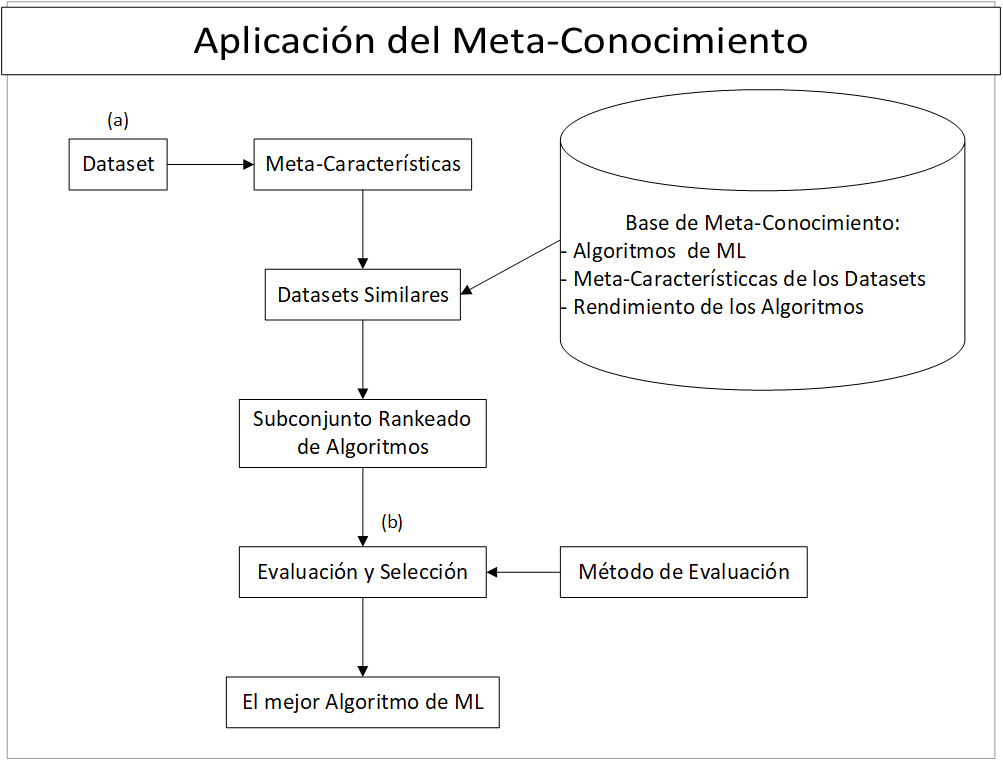
\includegraphics[scale=.5]{Figures/application.png}
	%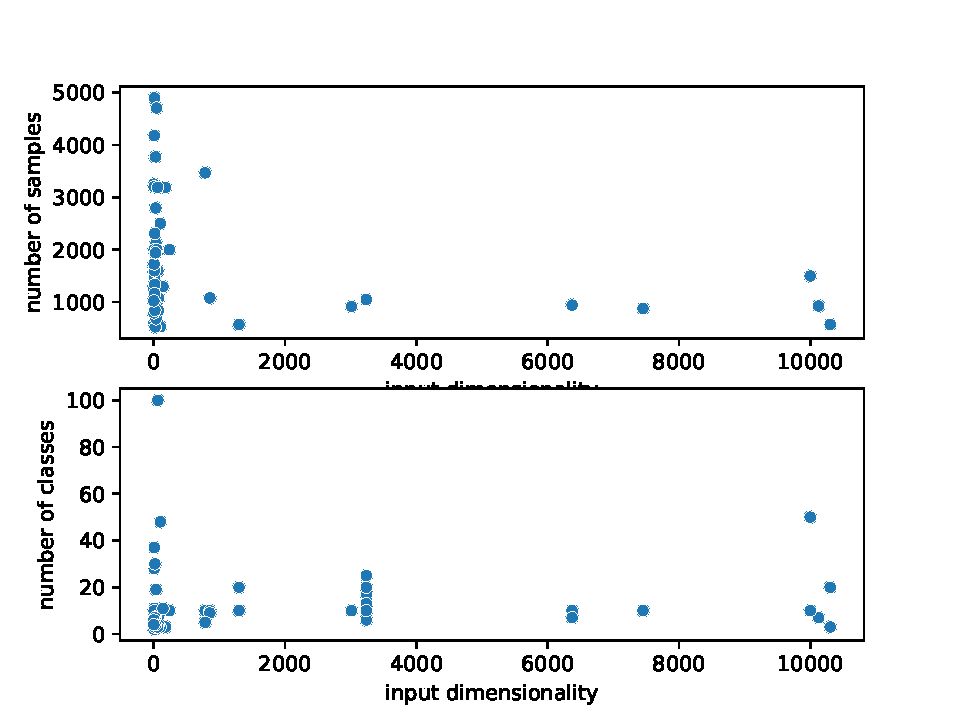
\includegraphics[scale=.60]{Figures/mtf scatterplot.pdf}
	\caption{Proceso de aplicación de meta-conocimiento. %Está compuesto por dos fases, en la primera fase (1) dado un nuevo dataset sus meta-características son extraídas y estas son analizadas para extraer de la base de meta-conocimiento los datasets similares, luego se obtiene un subconjunto ordenado de algoritmos. En la segunda fase (2) se busca en el espacio de búsqueda reducido a través de un proceso de evaluación para obtener el algoritmo con mejor rendimiento para el nuevo dataset.
		}
	\label{fig:application}
\end{figure}

\subsection{Aplicaciones de Meta-Learning}\label{subsec:mtl_aplications}

Meta-learning puede ser empleada en una variedad de configuraciones, con cierto desacuerdo en la literatura sobre lo que constituye exactamente un problema de meta-learning. Meta-learning es extremadamente útil en los casos donde es requerido un modelo de aprendizaje automático y hay poca cantidad de datos, ya que el modelo contiene muchos parámetros que no pueden ser estimados precisamente con pocos datos. Algunas de las aplicaciones comunes son en la investigación robótica, donde se espera que los robots tengan un mayor nivel de autonomía en IA, en el descubrimiento de drogas para manejar los datos de altas dimensiones con un tamaño de muestra pequeño y en la traducción de lenguajes raramente usados~\cite{peng2020comprehensive}. Además, meta-learning es ampliamente empleado en el problema de selección de algoritmos, sobre esta aplicación se profundiza en la Sección \ref{sec:metalearning-automl}.

Meta-learning constituye una solución factible para los problemas donde una definición específica de ``tarea'' y ``etiqueta'' puede ser claramente distinguida. Un sistema de meta-learning es flexible y puede ser integrado convenientemente con la mayoría de los algoritmos de aprendizaje automático para proporcionar soluciones factibles~\cite{peng2020comprehensive}. Para las tareas que son computacionalmente costosas, meta-learning presenta la opción de agregación o adaptación de los resultados anteriores para salvar recursos computacionales.
 
\section{AutoML}\label{sec:automl}

%\begin{itemize}
%	\item Introducir el tema de AutoML y su propósito
%\end{itemize}


%\begin{itemize}
%	\item[$\checkmark$] Definición de AutoML, quizá desde distintas perspectivas usando diferentes definiciones
%	\item[$\checkmark$] Explicar además varias de las subtareas de AutoML \begin{itemize}
%		\item[$\checkmark$] \textit{Automated feature enginineering}
%		\item[$\checkmark$] \textit{Automated model selection}
%		\item[$\checkmark$] \textit{Neural architecture search}
%	\end{itemize}
%\end{itemize}

\textit{Automated Machine Learning} (AutoML) o Aprendizaje de Máquinas Automático es el campo que se enfoca en los métodos que tienen el objetivo de automatizar diferentes etapas del proceso de aprendizaje automático. Como su nombre indica, AutoML es la intersección de dos campos: automatización y ML. Las soluciones de AutoML están recibiendo incrementalmente más atención tanto por la comunidad de ML como por los usuarios por las grandes cantidades de datos disponibles en todas partes y la falta de expertos de aprendizaje automático que puedan supervisar/asesorar el desarrollo de sistemas basados en ML~\cite{hutter2019autmlbook}.

La diferencia entre el aprendizaje automático clásico y AutoML es que en el primero, los humanos están grandemente involucrados en la configuración de las herramientas de aprendizaje realizando ingeniería de características, selección y evaluación de modelos. Como resultado, los humanos realizan la mayor parte del trabajo en las prácticas del aprendizaje automático. Sin embargo, en AutoML, todo esto puede ser hecho con programas de forma automática.

La comunidad de AutoML se ha centrado en resolver varias partes de un flujo de trabajo de aprendizaje automático estándar. Algunos ejemplos de estas partes o subtareas que son aplicadas en AutoML son:

\begin{description}
	\item[\textit{Automated Data Preparation} o Preparación Automática de Datos:] el flujo de trabajo de la preparación de datos está compuesto por 3 componentes: colección de datos, limpieza de datos e incremento de datos. La colección de datos es un paso necesario para construir un nuevo dataset o extender el dataset existente. El proceso de limpieza de datos es usado para filtrar los datos con ruido para que el entrenamiento del modelo no sea comprometido. El incremento de datos tiene un rol importante en mejorar la robustez del modelo y mejorar su rendimiento. Este paso es uno de los que más difícilmente son automatizados~\cite{he2021automl}.
	
	\item[\textit{Automated Feature Engineering} o Ingeniería Automática de Características:] el objetivo de ingeniería de características es construir más características para mejorar el rendimiento de aprendizaje cuando las características no son lo suficientemente informativas. Para esto se diseña un modelo que aprende de las características de entrada para construir nuevas características, con las cuales el algoritmo de aprendizaje automático obtiene un mejor rendimiento. Con la automatización de esta tarea se elimina parte de la asistencia humana para construir automáticamente nuevas características~\cite{he2021automl}.
	
%	\item[\textit{Automated Model Selection} o Selección Automática de Modelos:] el objetivo de la selección de modelos es encontrar un algoritmo de aprendizaje de máquinas adecuado para un dataset determinado. Hay muchos aspectos por los cuales un científico de datos se preocupa en la selección de algoritmos, tales como la complejidad computacional, diferencias en el tiempo de entrenamiento y si el algoritmo permite una entrada no lineal, y es útil considerar estos aspectos en la automatización. Para realizar esta tarea un sistema AutoML realiza una búsqueda sobre un conjunto de algoritmos disponibles, con el objetivo de determinar cuáles pertenecen al flujo óptimo dado un problema determinado.

	% \item[\textit{Model Evaluation} o Evaluación del Modelo:] Una vez que el modelo ha sido generado, su rendimiento debe ser evaluado. Un método intuitivo consiste en entrenar el modelo hasta que converja y entonces evaluar su rendimiento. Sin embargo, este método requiere un tiempo y unos recursos computacionales extensivos. Por lo tanto, existen varios métodos para acelerar el proceso de evaluación de modelos. Algunos ejemplos de estos métodos son \textit{early stopping} (explicar). El uso de \textit{Low fidelity} y de \textit{surrogate models} o modelos sustitutos son otras técnicas de evaluación que serán explicadas más adelante (poner link)
	
	\item [\textit{Neural Architecture Search} (NAS) o Búsqueda de Arquitecturas Neuronales:] el objetivo de NAS es encontrar una arquitectura de redes neuronales profundas con buen rendimiento en un dataset determinado. NAS ha sido usado para diseñar redes que están a la par o tienen mejores resultados que arquitecturas diseñados a mano~\cite{zoph2017learning, witsuba2019nas}. Aunque es una práctica común optimizar la arquitectura y las configuraciones de los hiperparámetros en secuencia, existe evidencia reciente de que deberían ser optimizadas en conjunto \cite{bischl2021hyperparameter}.
\end{description}

Sin embargo, los estudios recientes de AutoML buscan automatizar el flujo de algoritmos de aprendizaje automático entero~\cite{fuerer2015efficient, olson2019tpot, paszke2019pytorch, chen2018autostacker, swearingen2017atm}. Un flujo de algoritmos es una forma de codificar y automatizar el flujo de trabajo necesario para producir un modelo de aprendizaje automático. Los flujos de algoritmos de aprendizaje automático constan de varios pasos secuenciales que realizan desde la extracción de datos y el preprocesamiento hasta el entrenamiento y la implementación del modelo~\cite{web-mlpipe}.

\subsection{Definición del problema}\label{subsec:automl_problem_definition}

%\begin{itemize}
%	\item[$\checkmark$] Definir el problema de automl en términos de CASH
%	\item[$\checkmark$] Definir el problema de optimización de hiperparámetros (HPO) 
%	\item[$\checkmark$] Definir el problema de \textit{Combined Algorithm Selection and Hyperparameter tuning} (CASH)
%%	\item Definir el workflow de un sistema de AutoML \begin{itemize}
%%		\item Su entrada es un conjunto de datos, una métrica de optimización (poner ejemplos de métricas de optimización) y (generalmente) restricciones de tiempo.
%%		\item Su salida es un modelo (pipeline?) de machine learning con sus hiperpárametros.
%%		\item El sistema de AutoML está fundamentalmente definida por la técnica de optimización usada y la definición del espacio de búsqueda.  
%%	\end{itemize}
%\end{itemize}

Dos problemas importantes en AutoML son que ningún algoritmo de ML obtiene los mejores resultados en todos los datasets, también conocido como \textit{No Free Lunch Problem} \cite{wolpert1995no}, y que algunos métodos de aprendizaje automático dependen crucialmente de la optimización de hiperparámetros. Para la resolución de estos problemas AutoML se apoya de dos áreas o subtareas que constituyen su base: la selección de modelos (\textit{Model Selection}, MS)~\cite{thornton2013auto} y la optimización de hiperparámetros (\textit{Hyperparameter Optimization}, HPO)~\cite{fuerer2019hyperparameter}. La combinación de estas áreas se refiere al problema de AutoML como un problema de selección combinada de modelos y optimización de hiperparámetros (\textit{Combined Algorithm Selection and Hyperparameter Optimization}, CASH)~\cite{thornton2013auto}, que se describe en la presente sección.

\subsubsection{Selección de Modelos}

El objetivo de la selección de modelos es encontrar un algoritmo de aprendizaje automático adecuado para un dataset determinado. Hay muchos aspectos de los cuales un científico de datos se preocupa en la selección de algoritmos, tales como la complejidad computacional, diferencias en el tiempo de entrenamiento y si el algoritmo permite una entrada no lineal, y es útil considerar estos aspectos en la automatización. Para realizar esta tarea un sistema AutoML realiza una búsqueda sobre un conjunto de algoritmos disponibles, con el objetivo de determinar cuáles de ellos pertenecen al flujo óptimo de un problema determinado.

\begin{definition}
	Dado un conjunto A de algoritmos de aprendizaje automático y una cantidad limitada de datos $D = \{(x_i, y_1),..., (x_n, y_n)\}$, el objetivo de la selección de modelos es determinar el algoritmo $a^* \in A$ con un rendimiento óptimo general. Para una evaluación general se divide el conjunto de datos $D$ en dos conjuntos disjuntos $D_{train}$ y $D_{valid}$ para entrenamiento y validación respectivamente, se aprenden funciones $f_i$ al aplicar $a^*$ a $D_{train}$, y se evalúa el rendimiento de las funciones en $D_{valid}$. Más formalmente, el problema de selección de modelos consiste en encontrar

	\begin{equation}
		a^* = \underset{a \in A}{argmin} \dfrac{1}{k}\sum_{i=1}^K \textbf{L}(a, D_{train}, D_{valid})
	\end{equation}
	
	donde $L(a, D_{train}, D_{valid})$ es la pérdida de $a$ al ser evaluado en $D_{valid}$ y entrenado con $D_{train}$.
	
%	 El protocolo de validación puede tomar distintas formas; una de las opciones más populares es el cálculo del error de validación cruzada con una función de pérdida definida por el usuario.

\end{definition}

\subsubsection{Optimización de Hiperparámetros}

Los algoritmos de aprendizaje automático son altamente configurables por sus hiperparámetros (HP). Estos últimos a menudo influencian substancialmente el comportamiento y la velocidad del algoritmo y tienen que ser seleccionados con cuidado con el objetivo de alcanzar un rendimiento óptimo. Tanto para expertos como para no expertos, ajustar los hiperparámetros para optimizar el rendimiento del modelo puede ser una tarea difícil y tediosa, a menudo es bastante costosa y propensa a errores, especialmente cuando son seleccionados en un proceso de prueba y error. Los algoritmos de optimización de hiperparámetros (HPO) identifican automáticamente una configuración de hiperparámetros (HPC) buena para un algoritmo de ML, reduciendo así el esfuerzo humano. Por lo tanto, una de las tareas fundamentales de AutoML es ajustarlos para optimizar el rendimiento de los algoritmos de ML.

\begin{definition}
	Sean A el conjunto de algoritmos de aprendizaje automático y $a \in A$ un algoritmo con $N$ parámetros. Denotamos el dominio del n-ésimo parámetro como $\Lambda_n$ y el espacio de configuraciones como $\Lambda = \Lambda_1 \times \Lambda_2 \times ... \times \Lambda_x$. Un vector de hiperparámetros es denotado por $\lambda \in \Lambda$, y $a$, con sus hiperparámetros instanciados en $\lambda$, por $a_\lambda$.
\end{definition}


Existe gran variedad de dominios en los hiperparámetros, pueden tener valores continuos, discretos, booleanos o categóricos. Por ejemplo, el hiperparámetro de ritmo de aprendizaje de una red neuronal es continuo; la cantidad de capas es discreta y la decisión de eliminar \textit{stopwords} o no es booleana. 

Este espacio ya mixto puede desafortunadamente contener \textit{hiperparámetros dependientes} o \textit{condicionales}, lo que conlleva a un espacio de búsqueda jerárquico \cite{bischl2021hyperparameter}.

\begin{definition}
	Un hiperparámetro $\lambda_i$ se considera \textit{condicional} con $\lambda_j$ si $\lambda_i$ solo está activo cuando $\lambda_j$ toma un valor determinado de un subconjunto dado de $\Lambda_j$.
\end{definition} 

Por ejemplo, los parámetros que determinan las especificaciones de la tercera capa de una red neuronal profunda no son relevantes si la profundidad de la red tiene valor 1 o 2. Igualmente, los parámetros de un kernel polinomial de un SVM no son importantes si se usa un kernel diferente.

Estos hiperparámetros generalmente introducen dependencias en forma de árbol en el espacio de búsqueda, y en general pueden ocasionar dependencias representadas como grafos dirigidos acíclicos.


A causa de esta variedad en los espacios de hiperparámetros, los algoritmos de optimización, o no se aplican directamente, u operan sin aprovechar la estructura valiosa en el espacio de búsqueda.

Entonces según la definición de Feurer et al~\cite{fuerer2019hyperparameter}, dado un conjunto de datos $D$, el problema de HPO general está definido como:

$\underset{below}{above}$

\begin{equation}
	\lambda^* = \underset{\lambda \in \Lambda}{argmin} \textbf{E}_{(D_{train}, D_{valid}) \sim  D}\textbf{V}(L, a_\lambda, D_{train}, D_{valid}),
\end{equation}

donde $\textbf{V}(L, a_\lambda, D_{train}, D_{valid})$ mide la pérdida de un modelo generado por $a_\lambda$ en el conjunto de entrenamiento $D_{train}$ y evaluado sobre el conjunto $D_{valid}$. Al igual que en la selección de modelos, hay distintos métodos de validación que pueden ser usados para comprobar los resultados, uno de los más populares es la validación cruzada.

\subsubsection{AutoML como problema de CASH} 

El problema de resolver MS y HPO de forma independiente es que ningún algoritmo rinde mejor en todos los conjuntos de datos y existen algoritmos que dependen decisivamente de sus hiperparámetros. Afortunadamente, estos dos problemas pueden ser abordados como un problema de optimización simple, estructurado y conjunto:

\begin{definition}
	Sea $A = \{a^{(1)}, a^{(2)}, ..., a^{(k)}\}$ un conjunto de algoritmos con espacios de configuraciones asociados $\Lambda_1, ... \Lambda_k$. Sea D un conjunto de datos que se divide en $\{D_{train}^{(1)}, ..., D_{train}^{(k)}\}$ y $\{D_{valid}^{(1)}, ..., D_{valid}^{(k)}\}$ tal que $D^{(i)}_{train} = D\backslash D_{valid}^{(i)}$, para $i=1,...,k$. Finalmente, sea $L(a_\lambda^{(j)}, D_{train}^{(i)}, D_{valid}^{(i)})$ la pérdida del algoritmo $a^{(j)}$ en el dataset $D_{valid}$ cuando es entrenado en el dataset $D_{train}$. Luego, el problema de la \textsl{Selección Combinada de Modelos y Optimización de Hiperparámetros (CASH)} consiste en encontrar el algoritmo y la configuración de hiperparámetros que minimice la pérdida:
	
	\begin{equation}\label{cash}
	 a^*_{\lambda^*} \in \underset{a^{(j) \in A, \lambda \in \Lambda^{(j)}}}{argmin} \dfrac{1}{k} \sum_{i=1}^{k} L\left(a_\lambda^{(j)}, D_{train}^{(i)}, D_{valid}^{(i)}\right)
	\end{equation}
\end{definition}   

%En la práctica, una de las restricciones de las técnicas de optimización de CASH es el \textit{presupuesto de tiempo}. En particular, el objetivo del algoritmo de optimización es seleccionar y ajustar un algoritmo de aprendizaje de máquinas que puede lograr rendimiento casi óptimo en términos de métricas de evaluaciones definidas por el usuario (por ejemplo, accuracy, sensitivity, specificity, F1-score) dentro del \textit{presupuesto de tiempo} definido por el usuario.

En la práctica, el problema de CASH es reformulado como un solo problema de optimización de hiperparámetros jerárquico con el espacio de parámetros $\Lambda^{(1)}\cup ... \cup \Lambda^{(k)} \cup\{\lambda_r\}$, donde $\lambda_r$ es un nuevo hiperparámetro que selecciona entre los algoritmos $a^{(1)}, ..., a^{(k)}$. Todos los parámetros de cada subespacio $\Lambda^{(i)}$ se vuelven condicionales de $\lambda_r$ al ser inicializado como uno de los algoritmos $a^i$.
 
\subsection{Estrategias de Búsqueda}\label{subsec:automl_methods}

%\begin{itemize}
%	\item[$\checkmark$] Introducir esta sección
%	\item A lo largo de esta sección, mi idea es explicar los algoritmos que usan cada una de estas técnicas de optimización a medida que las describo, pero quizá sería un poco más organizado si hago otra subsección poniendo ejemplos de los sistemas de AutoML aparte para además no darle tanta importancia a los algoritmos de optimización (hmmm...)
%\end{itemize}

Con el objetivo de abordar el problema \ref{cash} el proceso de AutoML consta de tres componentes que definen el proceso de optimización:

\begin{description}
	\item[Espacio de Búsqueda:] precisa los algoritmos y todos los rangos válidos para sus hiperparámetros que son posibles soluciones para un problema de AutoML concreto. Además, se pueden optimizar combinaciones complejas de algoritmos, en cuyo caso las restricciones de compatibilidad entre algoritmos también son modeladas.
	\item[Estrategia de Búsqueda:] detalla como se explora el espacio de búsqueda, que puede ser de tamaño exponencial o ilimitado. Se ve afectado por el clásico problema de Exploración vs. Explotación, ya que se quieren encontrar soluciones de alto rendimiento rápidamente, pero se debe evitar converger prematuramente a regiones subóptimas de búsqueda.
	\item[Estrategias de Estimación de Rendimiento:] son mecanismos para estimar la capacidad predictiva de las soluciones encontradas por los sistemas de AutoML.
\end{description}

La estrategia de búsqueda es el proceso que sustituye la búsqueda de los hiperparámetros realizada por los humanos. Este procedimiento requiere tiempo y recursos considerables debido a los métodos de prueba y error que son necesitados para buscar el mejor modelo y su configuración de hiperparámetros. Por lo tanto, muchos métodos de optimización han surgido con el objetivo de acelerar esta búsqueda para liberar a los humanos de este tedioso proceso y para explorar el espacio de búsqueda definido de forma automática. Este proceso de optimización es el que pretende imitar el rol de los expertos y es el núcleo fundamental para resolver el problema de CASH. Por lo tanto, a continuación se realiza un estudio de las estrategias de búsquedas más usadas, ejemplificando su uso en distintos sistemas de AutoML.

% A diferencia de los parámetros del modelo que se aprenden durante el entrenamiento, el científico de datos establece los hiperparámetros del modelo antes de los aspectos de implementación de control y entrenamiento del modelo. Los hiperparámetros se pueden considerar como configuraciones de modelo. Estos deben ajustarse porque los hiperparámetros ideales para un conjunto de datos no serán los mismos en todos los conjuntos de datos.

\subsubsection{Grid Search y Random Search}

%\begin{itemize}
%	\item[$\checkmark$] Hablar de la necesidad de Grid Search y Random Search como métodos populares para el ajuste de hiperparámetros y del hecho de que son simples métodos de búsqueda que no hacen ninguna suposición sobre el espacio de búsqueda pero son muy ineficientes.
%	\item[$\checkmark$] Explicar en lo que consiste Grid Search
%	\item[$\checkmark$] Explicar en lo que consiste Random Search.
%	\item[$\checkmark$] Compararlos
%	\item[$\checkmark$] Poner ejemplos de sistemas que usan RS y GS (casi todos los hacen), hablar quizá de que estos métodos están implementados en sklearn
%\end{itemize}

Al ajustar los hiperparámetros de un algoritmo, \textit{Grid Search} y \textit{Radom Search} son métodos populares usados por su simplicidad y por el hecho de que no realizan suposiciones sobre el espacio de búsqueda. Cada configuración en el espacio de búsqueda pueden ser evaluados independientemente. Usualmente es ineficiente porque no explota el conocimiento ganado de evaluaciones pasadas.

\textit{Grid Search} (GS) es el proceso de discretizar cada hiperparámetro y evaluar exhaustivamente cada combinación de valores. Los valores numéricos de los hiperparámetros suelen estar espaciados equidistantemente en los intervalos en los que se define. Para los hiperparámetros categóricos, se consideran un subconjunto o todos los valores posibles. Es la manera más tradicional de ajustar hiperparámetros. Para obtener la configuración de hiperparámetros óptima, \textit{grid search} tiene que enumerar cada configuración posible en el espacio de búsqueda, lo que lo hace muy ineficiente. Por ejemplo, la búsqueda de 20 valores de parámetros diferentes para 4 parámetros requerirá 160.000 ensayos de validación cruzada. Esto equivale a 1.600.000 ajustes de modelo y 1.600.000 predicciones si se realiza validación cruzada 10 veces. Es extremadamente costosa en tiempo. Además, la discretización es necesaria cuando el espacio de búsqueda es continuo.

Por otro lado, \textit{Random Search} (RS) o búsqueda aleatoria configura una cuadrícula de valores de hiperparámetros y selecciona combinaciones aleatorias para entrenar el modelo. Esto permite controlar explícitamente el número de combinaciones de parámetros que se intentan. El número de iteraciones de búsqueda se pueden establecer en función del tiempo o los recursos.

%% RS a menudo tiene un rendimiento mucho mejor que GS en entornos de mayor dimensión. GS sufre directamente de la maldición de la dimensionalidad, ya que el número requerido de evaluaciones aumenta exponencialmente con el número de hiperparámetros para un número de valores de hiperparámetros fijo. Esto también parece ser cierto para RS a primera vista, y ciertamente necesitamos un número exponencial de puntos para cubrir bien el espacio. Pero en la práctica, los problemas de HPO a menudo tienen una dimensionalidad efectiva baja: el conjunto de hiperparámetros que influyen en el rendimiento suele ser un pequeño subconjunto de todos los hiperparámetros disponibles. Otra ventaja de RS es que se puede ampliar fácilmente con más muestras; por el contrario, el número de puntos en una cuadrícula debe especificarse de antemano y refinar la resolución de GS posteriormente es más complicado. Todo esto hace que RS sea preferible a GS y una base sorprendentemente sólida para HPO en muchos entornos prácticos.

GS y RS son métodos de fácil implementación, por lo que es común su uso para realizar la búsqueda de hiperparámetros. Ambos se encuentran implementados en una de las bibliotecas más populares de Python para el aprendizaje automático: \texttt{scikit-learn} \cite{scikit-learn}. Ambas técnicas evalúan los modelos dado un vector de hiperparámetros determinado usando validación cruzada. Requieren dos argumentos: una instancia del modelo que se quiere optimizar y un espacio de búsqueda donde a cada hiperparámetro se asocia los valores discretos o en el caso de RS la distribución para muestrear.

Uno de los primeros sistemas de AutoML, Hyperopt \cite{bergstra2013hyperopt}, ya utilizaba RS entre sus estrategias de búsquedas como \textit{baseline}, comparando este método con la Optimización Bayesiana. En Hyperopt el espacio de búsqueda está compuesto por expresiones estocásticas que siempre evalúan a una entrada válida para la función objetivo. Las expresiones estocásticas representan a los hiperparámetros. RS está implementada muestreando simplemente estas expresiones estocásticas.

Rafiki \cite{wang2018rafiki} es otro de los sistemas de AutoML que emplea RS como método de optimización de hiperparámetros. Rafiki ha sido introducido como un \textit{framework} distribuido que está basado en la idea de usar modelos previos que logran un buen rendimiento en las mismas tareas. Para la implementación de RS, Rafiki utiliza un umbral $\alpha$ que representa la probabilidad de elegir una inicialización aleatoria y $1 - \alpha$ representa la probabilidad de usar parámetros pre-entrenados. A medida que avanza el proceso de búsqueda $\alpha$ se disminuye gradualmente para disminuir la posibilidad de inicialización aleatoria.

Por otro lado, FLAML \cite{wang2021flaml} usa otra versión de RS que ha sido propuesta recientemente, el método de búsqueda directa aleatoria \cite{wu2021frugal}. El algoritmo utiliza una configuración de bajo costo como punto de partida. En cada iteración, toma muestras de una dirección en una esfera unitaria y luego decide si pasar a una nueva configuración a lo largo de la dirección muestreada (o la dirección opuesta) dependiendo del signo observado en el cambio de error de validación. El tamaño del paso de movimiento se ajusta de forma adaptativa (es grande al principio para acercarse rápidamente a la complejidad requerida) y se reinicia la búsqueda (desde puntos iniciales aleatorios) ocasionalmente para escapar de los óptimos locales.

\subsubsection{Optimización Bayesiana}


%\begin{itemize}
%	\item[$\checkmark$] Introducir quizá diciendo su popularidad como técnica de optimización
%	\item[$\checkmark$] Hablar de manera general en qué consiste el algoritmo de optimización, hablar de las funciones de adquisición y los modelos sustitutos, especialmente de su forma de equilibrar exploración (la evaluación de tantos conjuntos de hiperparámetros como sea posible) y explotación (asignar más recursos a los hiperparámetros más prometedores)
%	\item[$\checkmark$] Hablar de distintos tipos de modelos sustitutos y funciones de adquisición.
%	\item[$\checkmark$] Hablar de los sistemas: \begin{itemize}
%		\item Sin meta-learning: AutoWeka, HyperOpt, (\textit{maybe} AutoNet)
%		\item Con Meta-learning: 
%		\item Meta-features: Auto-Sklearn, SmartML 
%		\item Sin mf: Auto-Sklearn 2.0
%	\end{itemize}
%\end{itemize}

La optimización bayesiana, en inglés \textit{Bayesian Optimization} (BO), se ha vuelto cada vez más popular como técnica de optimización global para funciones costosas de caja negra, y específicamente para HPO.

BO es un algoritmo iterativo, cuya idea clave es modelar la asignación entre un conjunto de hiperparámetros $\lambda$ y da como resultado una estimación de su rendimiento $\hat{c}(\lambda)$ basado en valores de rendimiento observados encontrados en un archivo $A$ mediante regresión no lineal. Este modelo aproximado se denomina modelo sustituto, o modelo probabilístico, para el cual es normalmente utilizado un proceso gausiano o un bosque aleatorio. BO comienza en un archivo $A$ lleno de configuraciones evaluadas. Este archivo es normalmente generado a partir de una configuración de diseño inicial, típicamente muestreada al azar. BO luego usa el archivo para ajustar el modelo sustituto, que para cada $\lambda$ produce una estimación del rendimiento $\hat{c}(\lambda)$, así como una estimación de la incertidumbre del modelo $\hat{\sigma}(\lambda)$. Sobre la base de estas predicciones, BO establece una función de adquisición $u(\lambda)$ fácil de evaluar, cuyo resultado codifica una compensación entre explotación (el modelo sustituto predice que el candidato $\lambda$ tiene un valor rendimiento $\hat{c}$ bueno y bajo) y exploración (el modelo sustituto es muy incierto acerca del rendimiento, probablemente porque el área circundante no ha sido explorada minuciosamente).

\quad

\textbf{Modelos sustitutos}

\quad

Un modelo sustituto es una función que aproxima el comportamiento de la función objetivo lo más fielmente posible, y es computacionalmente más fácil de evaluar. La elección del modelo sustituto tiene una gran influencia en el rendimiento de BO y a menudo está relacionado con las propiedades del espacio de búsqueda $\Lambda$. 

Si $\Lambda$ es puramente numérico, los procesos gausianos (GPs)~\cite{rasmussen2005gaussian}, son los usados más a menudo~\cite{bischl2021hyperparameter}. Sin embargo, los procesos gausianos tiene una complejidad de tiempo de ejecución que es cúbica en el número de ejemplos, lo que puede resultar en una sobrecarga significativa cuando el archivo $A$ se vuelve grande.

Los bosques aleatorios (\emph{random forests}), utilizados más notablemente en SMAC (\emph{Sequential Model-based Algorithm Configuration})~\cite{hutter2011sequential}, también han mostrado buenos rendimientos como modelos sustitutos para BO. Su ventaja es su habilidad nativa para manejar hiperparámetros discretos y, con modificaciones menores, incluso los hiperparámetros dependientes sin la necesidad de preprocesamiento. Las implementaciones estándar de bosque aleatorio pueden manejar hiperparámetros dependientes al tratar los valores no factibles como faltantes. Los bosques aleatorios tienden a funcionar bien con archivos más grandes e introducen menos gastos generales que los GPs. %% SMAC usa la desviación estándar de las predicciones de los árboles como una estimación de incertidumbre heurística $\hat{\sigma}(\lambda)$,  sin embargo, existen alternativas más sofisticadas para proporcionar estimaciones no sesgadas. Dado que los árboles no son modelos espaciales basados en la distancia, el estimador de incertidumbre no aumenta cuanto más extrapolamos de los puntos de entrenamiento observados. Este podría ser una explicación de por qué GP supera a los sustitutos basados en árboles en la búsqueda en espacios puramente numéricos.

% Las redes neuronales o \emph{Neural Networks} (NN), han mostrado un buen rendimiento en particular con espacios de entrada no triviales, por lo que se consideran cada vez más como modelos sustitutos de BO. Los NN ofrecen implementaciones eficientes y versátiles que permiten el uso de gradientes para una optimización más eficiente de la función de adquisición. Los límites de incertidumbre en las predicciones se pueden obtener, por ejemplo, utilizando Redes Neuronales Bayesianas que combinan Redes Neuronales con un modelo probabilístico de los pesos de la red o regresión de base adaptativa donde solo se agrega un regresor lineal bayesiano a la última capa de la NN.

\quad

\textbf{Funciones de adquisición}

\quad

La función de adquisición equilibra la predicción del modelo sustituto $\hat{c}(\lambda)$ y su incertidumbre posterior $\hat{\sigma}(\lambda)$ para asegurar tanto la exploración de las regiones inexploradas del espacio de búsqueda $\Lambda$ como la explotación de las regiones que han tenido un buen rendimiento en las evaluaciones previas.

Diferentes funciones de adquisición han sido diseñadas para la optimización bayesiana, por ejemplo: probabilidad de mejora (\textit{probability of improvement}), búsqueda de entropía (\textit{entropy search}), límite de confianza superior (\textit{upper confidence bound}), límite de confianza inferior (\textit{lower confidence bound}) y mejora esperada (\textit{expected improvement}), siendo esta última una de las más populares.

%Basada en teoría de probabilidades, \textit{expected improvement} puede ser calculada relativa a la estimación actual del rendimiento óptimo. Suponiendo que nuestra métrica de rendimiento debería ser maximizada (por ejemplo, \textit{accuracy}, recobrado, etc), que para cualquier ajuste de combinación de hiperparámetros $\lambda$ tenemos la media predicha y el error estándar de esa métrica ($\mu(\lambda)$ y $\sigma(\lambda)$ respectivamente) y de los datos anteriores el mejor valor (medio) de rendimiento fue $m_{opt}$ \textit{expected improvement} es determinado usando:
%
%$$
% EI(\lambda, m_{opt}) = \delta(\lambda)\Phi\left(\frac{\delta(\lambda)}{\sigma(\lambda)}\right) + \sigma(\lambda)\phi\left(\frac{\delta(\lambda)}{\sigma(\lambda)} \right)
%$$
%
%Donde $\delta(\lambda) = m_{opt} - \mu(\lambda)$, la función  $\Phi(\cdot)$ es la función de distribución acumulativa y $\phi(\cdot)$ es la densidad normal estándar.
%
%El valor de $\delta(\lambda)$ mide cuán cerca estamos (en promedio) al mejor valor actual de rendimiento. Cuando se necesitan nuevos parámetros de ajuste candidatos, el espacio de $\theta$ es buscado por el valor que maximiza la mejora esperada.
%
\quad

\textbf{Ejemplos}

\quad

Esta estrategia de búsqueda ha sido ampliamente usada en diversos sistemas de AutoML. Auto-WEKA \cite{thornton2013auto}, es uno de los primeros sistemas de AutoML, introduciendo el problema de CASH y es uno de los ejemplos de sistemas que utilizan esta estrategia de búsqueda. En particular, usa \textit{Sequential Model-Based Optimization} (SMBO) o la Optimización Secuencial Basada en Modelos~\cite{hutter2011sequential}, un sistema versátil de optimización estocástica que puede trabajar explícitamente con hiperparámetros categóricos y continuos, y que puede explotar la estructura jerárquica derivada de los hiperparámetros condicionales. Auto-WEKA implementa dos algoritmos de SMBO que son adecuados para la tarea de la selección combinada de modelos y optimización de hiperparámetros: \textit{Sequential Model-based Algorithm Configuration} (SMAC)~\cite{hutter2011sequential} y \textit{Tree-structured Parzen Estimator} (TPE)~\cite{bergstra2011algorithms}. Empíricamente, compararon estos dos optimizadores para buscar en el espacio de hiperparámetros de 786 dimensiones de Auto-WEKA y terminaron recomendando la variante basada en el método de optimización bayesiana SMAC.

Hyperopt \cite{bergstra2013hyperopt} y Auto-Sklearn \cite{fuerer2015efficient} fueron dos sistemas posteriores de AutoML que también utilizan dos optimizadores bayesianos: SMAC y TPE respectivamente. Además de abordar el problema de CASH con SMAC, Auto-Sklearn emplea meta-learning para empezar la optimización bayesiana con buenas configuraciones \cite{fuerer2015initializing} evaluada en datasets similares. Auto-Sklearn además aplica \textit{ensemble learning}, construyendo \textit{ensembles} de los modelos evaluados con SMAC \cite{hutter2011sequential} para reducir el riesgo de hacer sobreajuste (\textit{overfitting}). \textit{Ensemble Learning} es un paradigma del aprendizaje automático donde múltiples modelos (a menudo llamados ``modelos débiles'') son entrenados para solucionar el mismo problema y combinarlos para obtener mejores resultados.

La optimización bayesiana ha sido también utilizada en redes neuronales modernas. Uno de las primeras herramientas en usar esta técnica fue Auto-Net~\cite{mendoza2016towards}, un sistema que automáticamente configura redes neuronales con SMAC siguiendo el mismo enfoque de AutoML que Auto-WEKA y Auto-Sklearn. Para la primera version de Auto-Net este sistema está implementado dentro de Auto-Sklearn añadiendo un nuevo componente de clasificación y regresión. Auto-Net está limitado a las redes neuronales completamente conectadas y utiliza la biblioteca de Python \texttt{Lasagne}~\cite{lasagne}, la cual está construida sobre Theano~\cite{theano2016theano}.

Otro sistema que usa BO para abordar el problema de NAS es Auto-Keras \cite{jin2019auto}. En esta herramienta se utiliza la optimización bayesiana para guiar el morfismo de la red para una búsqueda efectiva de arquitecturas neuronales. Como modelos sustitutos usan procesos gausianos (GPs) y como funciones de adquisición \textit{Upper Confidence Bound} (Límite de Confianza Superior).

\subsubsection{Optimización \textit{Multifidelity}}


%\begin{itemize}
%	\item[$\checkmark$] Introducir este concepto mediante su necesidad de uso para las redes neuronales.
%	\item[$\checkmark$] Explicar de forma concreta en que consiste el método de optimización.
%	\item[$\checkmark$] Hablar de AutoPytorch como ejemplo de sistema de AutoML (usa mtl sin meta-features)
%\end{itemize}

La optimización bayesiana es popular para optimizar los objetivos de caja negra que consumen mucho tiempo. No obstante, para el ajuste de hiperparámetros en redes neuronales profundas, el tiempo necesario para evaluar el error de validación, incluso para unos pocos ajustes de hiperparámetros, sigue siendo muy costosa. La optimización de \textit{multifidelity} promete alivio al usar \emph{proxies} más baratos para tales objetivos, por ejemplo, error de validación para una red entrenada usando un subconjunto de puntos de entrenamiento o menos iteraciones de las requeridas para la convergencia~\cite{wu2019practical}.

El concepto de \textit{Multifidelity} en HPO se refiere a todos los enfoques de ajuste de hiperparámetros que pueden manejar de manera eficiente a un modelo con un hiperparámetro de presupuesto $\lambda_{budget}$ como un componente del espacio de hiperparámetros $\Lambda$ que influye en el costo computacional del procedimiento de ajuste de una manera monótonamente creciente. Suponemos conocer las restricciones de $\lambda_{budget}$ en forma de límite inferior y superior. Por lo general, se asume que más presupuesto es mejor en términos de rendimiento predictivo (aunque, naturalmente, más costoso), pero esto puede propiciar que ocurra sobreajuste. Además, se supone que la relación entre el presupuesto y el rendimiento de la predicción cambia de forma algo suave, por lo que al evaluar múltiples configuraciones de hiperparámetros con un presupuesto pequeño, esto proporciona al menos un indicador con respecto a su clasificación cuando se evalúa con el presupuesto completo. Normalmente, esto implica un procedimiento de ajuste secuencial, donde $\lambda_{budget}$ es, por ejemplo,  el número de pasos de descenso de gradiente. % Otra opción, de aplicación general, es realizar una submuestra de los datos de formación del 0\% al 100\% antes de la formación y tratar esto como control de presupuesto. 

Los algoritmos de HPO que explotan dicho parámetro $\lambda_{budget}$, generalmente gastan el presupuesto en configuraciones de hiperparámetros baratos antes para la exploración y se concentran	 en los más prometedores más tarde, se denominan métodos de \textit{multifidelity}.

El ejemplo más notable del uso de esta estrategia es Auto-Pytorch \cite{zimmer2021auto}. \textit{Auto-PyTorch Tabular} es un sistema de AutoML dirigido a los datos tabulares que realiza la optimización \textit{multifidelity} en un espacio conjunto de parámetros de arquitectura e hiperparámetros de entrenamiento para redes neuronales. Auto-PyTorch Tabular es el sucesor de Auto-Net \cite{mendoza2016towards} y combina varios enfoques del estado del arte, desde optimización \textit{multifidelity} a \textit{ensemble learning} y meta-learning para una selección impulsada por los datos con el objetivo de seleccionar configuraciones iniciales para inicializar la optimización. Una elección importante en la configuración de la optimización \textit{multifidelity} es el tipo de presupuesto usado para crear las tareas \textit{proxy}. En esta herramienta eligen el número de las épocas (\textit{epochs}) de entrenamiento como su presupuesto por su generalidad e interpretabilidad. La optimización \textit{multifidelity} utilizada en Auto-Pytorch usa BOHB \cite{falkner2018bohb} para encontrar configuraciones con buenos rendimientos. BOHB combina la optimización bayesiana (BO) con \textit{Hyperband} (HP) \cite{li2018hyperband} y se ha demostrado que supera BO y HB en muchas tareas.

\subsubsection{Algoritmos Evolutivos}


%\begin{itemize}
%	\item[$\checkmark$] Introducción de los algoritmos evolutivos
%	\item[$\checkmark$] Definir conceptos importantes como \textit{individuos}, \textit{población} y sus principales operaciones \textit{mutation} y \textit{crossover}. Explicarlos en la terminología de HPO
%	\item[$\checkmark$] Hablar un poco de sus desventajas y propiedades.
%	\item[$\checkmark$] Mencionar los distintos paradigmas de los algoritmos evolutivos, para hacer hincapié en varios usados en los sistemas de AutoML: GGA, GA, PGE
%	\begin{itemize}
%	\item[$\checkmark$] Al explicar estos algoritmos concretos, hablar de los distintos sistemas de AutoML
%	\item[$\checkmark$] EA: Autostacker 
%	\item[$\checkmark$] GP: TPOT. No tiene mtl, pero hay trabajos incorporándolo, explicarlos.
%	\item[$\checkmark$] GGA: Auto-MEKA\_GPP, RECIPE (sin mtl)
%	\item PGE: Auto-GOAL sin mtl
%	\end{itemize}
%\end{itemize}

Un algoritmo evolutivo (EA) es un subconjunto de la computación evolutiva, un algoritmo genérico de optimización metaheurística basado en la población. Un EA utiliza mecanismos inspirados en la evolución biológica, como la reproducción, la mutación, la recombinación y la selección. Las soluciones candidatas al problema de optimización juegan el papel de individuos en una población, y la función de aptitud determina la calidad de las soluciones. La evolución de la población tiene lugar luego de la aplicación repetida de los operadores anteriores (reproducción, mutación, recombinación y selección).

En un algoritmo evolutivo, una \textit{población} de soluciones candidatas (llamadas individuos, criaturas o fenotipos) en un problema de optimización evoluciona hacia mejores soluciones. Cada solución candidata tiene un conjunto de propiedades (sus cromosomas o genotipo) que se pueden mutar y alterar.

La evolución generalmente comienza a partir de una población de individuos generados aleatoriamente y es un proceso iterativo, con la población en cada iteración llamada \textit{generación}. En cada generación, se evalúa la aptitud de cada individuo de la población; la aptitud suele ser el valor de la función objetivo en el problema de optimización que se resuelve. Los individuos más aptos se seleccionan estocásticamente de la población actual, y el genoma de cada individuo se modifica (recombina y posiblemente muta al azar) para formar una nueva generación. La nueva generación de soluciones candidatas se utiliza luego en la siguiente iteración del algoritmo. Por lo general, el algoritmo termina cuando se ha producido un número máximo de generaciones o se ha alcanzado un nivel de aptitud satisfactorio para la población.

En la terminología de la optimización de hiperparámetros un \textit{individuo} es una configuración de hiperparámetros única, la \textit{población} es un conjunto de configuraciones de hiperparámetros actualmente mantenido y la \textit{aptitud} de un individuo es su error de generalización. La mutación es el cambio (aleatorio) de uno o unos pocos valores de hiperparámetros en una configuración. El cruce crea una nueva configuración de hiperparámetros mezclando aleatoriamente los valores de otras dos configuraciones.

% Los EA estaban limitados a espacios numéricos enteros en su formulación original, pero pueden extenderse fácilmente para manejar espacios mixtos tratando componentes de diferentes tipos de forma independiente, por ejemplo, agregando un valor aleatorio normalmente distribuido a hiperparámetros de valor real mientras se agrega la diferencia de dos valores geométricamente distribuidos a hiperparámetros con valores enteros. Al definir operaciones de mutación y cruce que operan en estructuras de árbol o gráficos, es incluso posible realizar la optimización de \emph{pipelines} de preprocesamiento o arquitecturas de redes neuronales utilizando algoritmos evolutivos.

Los algoritmos evolutivos a menudo funcionan bien al aproximar soluciones a todo tipo de problemas porque, idealmente, no hacen ninguna suposición sobre la función de aptitud subyacente. % En la mayoría de las aplicaciones reales de EA, la complejidad computacional es un factor prohibitivo. De hecho, esta complejidad computacional se debe a la evaluación de la función de aptitud. La aproximación al fitness es una de las soluciones para superar esta dificultad.

Un ejemplo de uso de los algoritmos evolutivos se encuentra en Autostacker \cite{chen2018autostacker}. Autostacker combina una arquitectura innovadora jerárquica de \textit{stacking} y EA para realizar la búsqueda de parámetros de forma eficiente. Encuentra combinaciones innovadoras y estructuras de modelos de aprendizaje automático en vez de seleccionar un solo modelo y optimiza sus hiperparámetros. Para esto está inspirado en el método \textit{stacking} de \textit{ensemble learning}~\cite{wolpert1992stacked, breiman1996stacked}. La idea de \textit{stacking} es aprender de diferentes ``modelos débiles'' y combinarlos entrenando un meta-modelo para generar predicciones basadas en las múltiples predicciones retornadas por estos ``modelos débiles''. Por otro lado, EA les permite encontrar buenas soluciones en un espacio grande de variables. Además, explotando la naturaleza paralela de los algoritmos evolutivos, Autostacker encuentra rápidamente buenos candidatos de flujos de algoritmos.

TPOT \cite{olson2019tpot} optimiza flujos de algoritmos mediante una versión de programación genética (\textit{genetic programming}), una técnica muy conocida en la programación evolutiva para la construcción automática de programas. En la programación genética las soluciones están en la forma de programas de computadoras, y su aptitud está determinada por su habilidad para resolver un problema computacional. Una diferencia en el espacio de búsqueda de TPOT, en comparación con el resto de los sistemas mencionados, es que permite el uso de muchas copias de un dataset, el cual es procesado en paralelo por diferentes métodos de preprocesamiento y combinados con posterioridad. Además, TPOT considera una selección Pareto (NSGA-II) \cite{NSGA-II} para realizar la búsqueda multiobjetivo. Dos objetivos separados son considerados: maximizar la medida de precisión del flujo de trabajo y minimizar la complejidad total del mismo, que está dado por el número de operadores del flujo de trabajo, con el objetivo de evitar el sobreajuste.

Otro ejemplo lo constituye RECIPE \cite{de2017recipe}, el cual supera las debilidades de los otros \textit{frameworks} basados en algoritmos evolutivos anteriores, tales como generación de individuos inválidos, y organiza un gran número de posibles métodos de preprocesamiento de datos y de clasificación adecuados en una gramática. Para esto hace uso de un enfoque de Programación Genética basada en Gramáticas (GPP). Esta gramática permite dirigir la búsqueda, restringiendo las operaciones de mutación y cruzamiento. La estructura de la gramática le permite a RECIPE evitar, a diferencia de TPOT, la generación de flujos de algoritmos inválidos, y puede acelerar la búsqueda.

Otra herramienta de AutoML que utiliza GPP como estrategia de búsqueda es $Auto-MEKA_{GPP}$ \cite{de2018automated}. $Auto-MEKA_{GPP}$ está diseñada para resolver el problema de \textit{Multi-Label Classification} (MLC) y se apoya en la herramienta MEKA~\cite{MEKA}, la cual ofrece un número de algoritmos de MLC. En MLC, cada ejemplo puede ser asociado con una o más etiquetas de clase, lo que hace los problemas de MLC más difíciles que los problemas de clasificación convencionales, que poseen una sola etiqueta (\textit{Single Label Classification}, SLC). Mediante GPP, $Auto-MEKA_{GPP}$ es capaz de manejar la naturaleza jerárquica compleja del espacio de búsqueda de MLC mientras evita la generación de soluciones inválidas. Sin embargo, en el trabajo se enfocan en la búsqueda de algoritmos y sus hiperparámetros, no en flujos de trabajo completos. Esto se debe a que el espacio de búsqueda de MLC es mucho más grande que el espacio de búsqueda de SLC.

%\begin{itemize}
%	\item AUTOGOAL (debería hablar de ella aquí, o debería hablar de ella cuando hable de mi propuesta?s)
%\end{itemize}

AutoGOAL~\cite{autogoal} es un sistema de AutoML que destaca por su capacidad de abordar diferentes dominios combinando de forma transparente técnicas y herramientas dispares. AutoGOAL usa como método de optimización la Evolución Probabilística Gramatical o \textit{Probabilistic Grammatical Evolution}~\cite{pge2015} (PGE). El espacio de búsqueda en AutoGOAL se compone de un grafo $G_A$ dirigido y acíclico, donde cada nodo representa un algoritmo. Las aristas se definen entre algoritmos con tipos de entrada/salida compatibles. Dado un problema con un tipo de entrada y salida específico, se le añaden dos nodos ficticios, Entrada y Salida, al grafo $G_A$, que representan los tipos de entrada y salida del problema. En este grafo cualquier camino que comience en el nodo Entrada y termine en el nodo Salida representa un flujo que resuelve dicho problema. En AutoGOAL sobre el grafo de algoritmos $G_A$ de un problema específico se realiza un proceso de optimización para descubrir los mejores flujos válidos mediante generación aleatoria. Este proceso consiste en un ciclo de generación y evaluación utilizando una gramática construida a partir de $G_A$, dirigida por un modelo probabilístico $\sigma$.


\subsubsection{Aprendizaje por refuerzo}

%\begin{itemize}
%	\item[$\checkmark$] Introducir este método como algoritmo de optimización
%	\item[$\checkmark$] Hablar de la retroalimentación retardada: las retroalimentaciones (la recompensa y el estado) no necesitan ser devueltos inmediatamente una vez que se toma una acción pero una arquitectura solo se puede evaluar después de que se componga toda su estructura
%	\item[$\checkmark$] Explicar su desventaja de que consume gran cantidad de datos
%	\item[$\checkmark$] Hablar de los sistemas que usan Reinforcement Learning: AlphaD3M (mtl con meta-features)
%\end{itemize}

El aprendizaje por refuerzo (RL), como estrategia de búsqueda, consiste en entrenar un agente que realiza modificaciones sobre una solución con el objetivo de maximizar una recompensa que depende del rendimiento de dicha solución. Es un marco de optimización muy general y sólido, que puede resolver problemas con retroalimentación retardada. A diferencia de los métodos anteriores, las retroalimentaciones (es decir, la recompensa y el estado) no necesitan ser devueltos inmediatamente una vez que se toma una acción. Se pueden devolver después de realizar una secuencia de acciones. 

% El rendimiento de una arquitectura solo se puede evaluar después de que se componga toda su estructura, lo que implica una recompensa retrasada. Debido a las retroalimentaciones retrasadas, AutoML con aprendizaje por refuerzo consume una gran cantidad de datos y es necesario explorar métodos más eficientes. Algunos esfuerzos actuales para abordar estos problemas son el aprendizaje de arquitecturas transferibles a partir de conjuntos de datos más pequeños y la reducción del espacio de búsqueda compartiendo parámetros.

Esta estrategia es usual en la búsqueda de arquitecturas de redes neuronales (NAS), donde el agente puede realizar acciones como añadir, quitar o modificar una capa, o sus hiperparámetros. Las propuestas difieren en cómo representan la política del agente, y cómo la optimizan.

Un ejemplo del uso de esta estrategia se encuentra en Alpha3DM \cite{drori2018alphad3m}. Alpha3DM es un sistema de aprendizaje automático basado en \textit{meta reinforcement learning} usando una secuencia de modelos con auto juego (\textit{self play}). Inspirado en AlphaZero \cite{alphazero}, el jugador iterativamente construye un flujo seleccionando entre un conjunto de acciones, entre las cuales se encuentran inserción, eliminación y reemplazo de partes del flujo de algoritmos. Alpha3DM utiliza una red neuronal (específicamente, un LSTM (\textit{Long Short-Term Memory}) para predecir el rendimiento de un flujo y las probabilidades de acción, junto con Monte-Carlo Tree Search (MCTS), el cual toma decisiones fuertes basadas en la red.

\subsubsection{Multi-Armed Bandit}


%\begin{itemize}
%	\item[$\checkmark$] Introducir el problema de MAB, mencionar que es un caso particular de RL
%	\item[$\checkmark$] Explicar la solución del problema en el contexto de la optimización de hiperparámetros
%	\item Hablar de los sistemas que usan MAB:
%	\begin{itemize}
%		\item ATM usa BO y MAB Híbrido (explicar como cambia el algoritmo). Usa meta-learning
%		\item Alpine Meadow usa cost-based MAB con BO (explicar como cambia el algoritmo). Usa meta-learning con meta-features
%	\end{itemize}
%\end{itemize}

\textit{Multi-Armed Bandit} (MAB) es un problema en el que se debe asignar un conjunto limitado fijo de recursos entre diferentes opciones de una manera que maximice su ganancia esperada, cuando las propiedades de cada opción se conocen solo parcialmente en el momento de la asignación, y pueden entenderse mejor a medida que pasa el tiempo o mediante la asignación de recursos a la elección. Este es un problema clásico de aprendizaje por refuerzo que ejemplifica el dilema de compensación de exploración-explotación.

El problema de MAB puede definirse de la siguiente forma en el contexto de HPO:

\begin{definition}

Dado un conjunto de acciones (denominados en la formulación del algoritmo ``brazos'') $a \in A$, un presupuesto de tiempo $T$ y las distribuciones de recompensa $D$ que son desconocidas e independientes, en cada ronda $t \in [T]$:

\begin{enumerate}
	\item Un algoritmo elige una acción $a \in A$
	\item Los algoritmos observan una recompensa de la acción elegida $a_t$
\end{enumerate}

El objetivo es encontrar el algoritmo que mejor aproxima la solución con la menor pérdida de recompensa.

\end{definition}

Específicamente, cada acción $a_t$ es asociada con una configuración de hiperparámetros $\lambda$ y la recompensa (estocástica) por seleccionar un conjunto de hiperparámetros está definido en términos de error en las predicciones.

ATM \cite{swearingen2017atm} constituye en ejemplo de esta estrategia. ATM es un servicio de AutoML multi-usuario que puede ser desplegado en cualquier infraestructura, ya sea la nube o un \textit{cluster}. En ATM un usuario puede decidir entre dos métodos de optimización: 1) un sistema de optimización híbrida bayesiana y \textit{multi-armed bandit} y 2) un sistema de recomendación de modelos que funciona explotando las técnicas de modelación de los rendimientos anteriores en una gran variedad de dataset. El aprendizaje \textit{bandit} empleado en este sistema modela cada hiperpartición. Una hiperpartición define un conjunto ajustable de hiperparámetros condicionales, como una acción $a$. Dado que cada acción, cuando es elegida, proporciona una recompensa aleatoria elegida de la distribución subyacente, el propósito de MAB es decidir cuál acción seleccionar para maximizar la recompensa a largo plazo, revaluando la decisión después de que cada recompensa es observada. En el contexto de ATM, cada hiperpartición es tratada como una acción con su propia distribución de recompensas. A medida que pasa el tiempo, aprende más sobre la distribución, y balancea exploración y explotación eligiendo las hiperparticiones más prometedoras para formar los clasificadores. La optimización bayesiana es usada dentro de cada hiperpartición, usando como modelos sustitutos Procesos Gausianos (GPs), para identificar los mejores hiperparámetros dado el rendimiento de los clasificadores ya construidos para esa hiperpartición. ATM soporta 2 funciones de adquisición: \textit{Expected Improvement} y \textit{Expected Improvement per Time} \cite{snoek2012practical}.

\textit{Alpine Meadow} \cite{shang2019democratizing} ha sido recientemente introducido como una herramienta interactiva de AutoML. Además de su interoactividad se destaca por su enfoque de diseño sistemático y algorítmico. Por un lado se aprovecha de ideas de \textit{optimización de consultas} y por otro lado muestra estrategias nuevas de poda combinando \textit{Multi-Armed Bandits} basado en costo y Optimización Bayesiana. MAB es utilizada para modelar el proceso de selección de un flujo de trabajo general basado en la historia. La idea principal del algoritmo seguido es la siguiente:
\begin{enumerate}
	\item Inicialización: Tiene una acción para cada solución general (basado en la tarea y el dataset) ejecutados en el pasado y presentan una puntuación para cada acción basada en la experiencia pasada.
	\item Selección: Selecciona una acción (es decir, solución) para ejecutar aleatoriamente pero de forma proporcional a la puntuación. Cuando la ejecución se haya terminado,
	\item Guardar Historia: Guardar el resultado en el registro de la historia.
	\item Ajustar Puntuaciones: Ajustar las puntuaciones consecuentemente, y el proceso se repite a partir del paso 1
\end{enumerate}

 % Toma prestado de la optimización de consultas la creación de espacios de búsqueda basado en reglas

\subsubsection{Monte Carlo Tree Search (MCTS)}

%\begin{itemize}
%	\item[$\checkmark$] Introducir el algoritmo
%	\item[$\checkmark$] Explicar los pasos en los que consiste MCTS: selección, expansión, simulación y backpropagation.
%	\item[$\checkmark$] Mencionar como MCTS extiende el algoritmo de MAB [link de mosaic]
%	\item[$\checkmark$] Ejemplificar la adaptación del procedimiento estándar de MCTS al problema de HPO 
%	\item[$\checkmark$] Poner ejemplos de sistemas
%	\item MOSAIC: usa meta-learning con meta-features
%\end{itemize}

Monte Carlo Tree Search (MCTS) es un algoritmo de búsqueda heurística para algunos tipos de procesos de decisión. El enfoque de MCTS es en el análisis de los movimientos más prometedores, expandiendo el árbol de búsqueda basado en un muestreo aleatorio del espacio de búsqueda. Cada ciclo de evaluación consiste en construir una solución completa, que se traduce en descender por una rama del árbol del espacio de búsqueda. En un algoritmo de Monte Carlo es necesario definir cómo se escoge el siguiente nodo a evaluar, lo que conlleva un balance entre exploración y explotación. A medida que se explora el espacio de búsqueda, se descubre qué decisiones en niveles superiores tienen un mejor rendimiento y se sesga la búsqueda hacia esas regiones del espacio. Para que esta estrategia sea efectiva, el espacio de búsqueda debe estar estructurado de forma que las decisiones más importantes ocurran antes.



%Cada ronda en MCTS consiste en 4 pasos:
%\begin{description}
%	\item[Selección:] comienza desde la raíz \textit{R} y selecciona los nodos secundarios sucesivos hasta que se alcance un nodo hoja \textit{L}. La raíz es el estado actual del juego y una hoja es cualquier nodo que tenga un hijo potencial a partir del cual aún no se ha iniciado ninguna simulación (reproducción). % La siguiente sección dice más sobre una forma de sesgar la elección de los nodos secundarios que permite que el árbol del juego se expanda hacia los movimientos más prometedores, que es la esencia de la búsqueda del árbol de Monte Carlo.
%	\item[Expansión:] a menos que \textit{L} termine el juego de manera decisiva (por ejemplo, ganar/perder/empatar) para cualquiera de los jugadores, crear uno (o más) nodos secundarios y elija un nodo \textit{C} entre ellos. Los nodos secundarios son cualquier movimiento válido desde la posición del juego definida por \textit{L}.
%	\item[Simulación:] Completa una reproducción aleatoria del nodo $C$. Este paso a veces también se denomina $playout$ o $rollout$. Un \textit{playout} puede ser tan simple como elegir movimientos aleatorios uniformes hasta que se decida el juego (por ejemplo, en el ajedrez, el juego se gana, se pierde o se empata).
%	\item[\textit{Backpropagation}:] usa el resultado del \textit{playout} para actualizar la información en los nodos en la ruta de \textit{C} a \textit{R}. 
%\end{description}

MCTS extiende el algoritmo de \textit{Multi-Armed Bandits} (MAB) a espacios de búsqueda estructurados como árboles. Un problema MAB define un problema de RL con un solo estado. MCTS relaja esta limitación de un solo estado y es conocido por ser un enfoque de RL eficiente~\cite{rakotoarison2019automated}.

MOSAIC~\cite{rakotoarison2019automated} constituye un ejemplo de uso de esta estrategia. MOSAIC utiliza MCTS para resolver eficientemente la optimización de flujos de algoritmos, que puede ser visto como un proceso de decisión secuencial. Por otro lado, emplea la Optimización Bayesiana para resolver el problema del ajuste de hiperparámetros. Estos dos enfoques son acoplados en MOSAIC a través de un modelo sustituto. Este modelo sustituto no es usado solamente para guiar la búsqueda local de los hiperparámetros, también es incorporado en el núcleo de la búsqueda de MCTS de la mejor estructura de los algoritmos utilizados.

%Un ejemplo de adaptación del procedimiento estándar de MCTS al problema de HPO es el llevado a cabo por MOSAIC \cite{rakotoarison2019automated} que sigue la siguiente estrategia:
%
%\begin{itemize}
%	\item El camino del árbol del nodo raíz a un node interno representa una solución parcial
%	\item  En cada nodo no-terminal, la elección del nodo hijo es realizado usando la regla UCB (\textit{Upper Confidence Bound}) en el caso finito, seleccionando el nodo hijo que maximiza: 
%	$$
%	 \mu_i + c\sqrt{\frac{logN}{n_i}}
%	$$
%	donde $\mu_i$  es el valor del nodo $i$, $N$ es el número de veces que el nodo padre fue visitado, $n_i$ es el número de veces que el nodo $i$ es visitado, y $c$ es la constante dependiente del problema que equilibra exploración y explotación.
%	\item Cuando se alcanza los límites del árbol visitado, una estrategia de \textit{rollout} es aplicada hasta alcanzar un nodo terminal y calcular la recompensa asociada.
%	\item La recompensa asociada al camino completo del árbol (nodo terminal, solución completa \textit{m}) es calculada.
%	\item Después de la evaluación del nodo terminal, la recompensa es propagada hacia atrás (\textit{backpropagated}) para actualizar el valor en cada nodo visitado del camino del árbol; este valor apoyará la elección entre los nodos hijos en el siguiente recorrido por el árbol.
%\end{itemize}

\subsubsection{Descenso por Gradientes}

%\begin{itemize}
%	\item[$\checkmark$] Introducir el método hablando de los problemas de su uso para HPO
%	\item[$\checkmark$] Explicar cómo se usa en la solución del problema
%	\item[$\checkmark$] Hablar de HyperGD, y poner el ejemplo de Oracle, que es un sistema que usa este método de optimización. Usa meta-learning
%\end{itemize}

Los problemas de HPO suelen ser complejos, ya que en general el objetivo no suele ser diferenciable o incluso continuo. Cada hiperparámetro que está definido por un conjunto discreto introduce superficies no suaves. Además, en general el problema de HPO no es convexo. Toda la teoría de convergencia de \textit{Gradient Descent} (GD) (Descenso por Gradientes) asume que el problema subyacente es convexo. Por lo tanto, el descenso por gradientes no es tan popular como los métodos anteriores~\cite{dai2020lower}. Sin embargo, centrándose en alguna función de pérdida diferenciable, los hiperparámetros continuos se pueden optimizar mediante el descenso por gradientes.

En comparación con los métodos anteriores, los gradientes ofrecen la información más precisa de donde se ubican las mejores configuraciones. A diferencia de los problemas de optimización tradicionales, cuyos gradientes se pueden derivar explícitamente a partir del objetivo, en los problemas de AutoML los gradientes deben calcularse numéricamente.

%Por lo general, esto se puede hacer con métodos de diferenciación finita pero con costos elevados. Para algunos métodos tradicionales de aprendizaje automático, por ejemplo, regresión logística y SVM, se propone el gradiente aproximado para buscar hiperparámetros continuos. El cálculo de gradientes exactos se basa en la convergencia del entrenamiento del modelo. A través de un gradiente inexacto, los hiperparámetros se pueden actualizar antes de que converja el entrenamiento del modelo, lo que hace que el método de descenso del gradiente sea más eficiente.

Otra forma de calcular gradientes es mediante el aprendizaje reversible \cite{maclaurin2015gradient} (también denominado diferenciación automática). Calcula gradientes con la regla de la cadena, que también se utiliza en el proceso de retropropagación del entrenamiento de la red. Se ha aplicado en la búsqueda de hiperparámetros de aprendizaje profundo~\cite{maclaurin2015gradient, franceschi2017forward}. 

Oracle AutoML~\cite{OracleAutoML} es un ejemplo de esta estrategia de búsqueda. Para la optimización de hiperparámetros usa específicamente HyperGD, que está basado en gradientes altamente paralelos que realizan una optimización asincrónica en diferentes dimensiones de hiperparámetros en paralelo. La característica más destacada de Oracle AutoML es que es libre de iteraciones, diseñado no solo para proveer modelos precisos, sino también en un tiempo de ejecución más pequeño. Para liberar las etapas del aprendizaje automático de iteraciones emplea modelos proxy, que son meta-aprendidos, y que tienen el objetivo de predecir el rendimiento relativo de algoritmos y subconjuntos de datos. % Además, selecciona una muestra representativa de un dataset, junto con la fila y las dimensiones de las características, optimizadas por un algoritmo seleccionado. La reducción de datos adaptativos acelera la optimización de hiperparámetros con un impacto mínimo en el rendimiento predictivo de los modelos.

\subsubsection{Filtrado Colaborativo}

%\begin{itemize}
%	\item[$\checkmark$] Introducir este método, quizá hablando de cómo no es una técnica de optimización pero se usa para la selección de modelos
%	\item[$\checkmark$] Explicar en que cosiste este método
%	\item[$\checkmark$] Explicar el método en el contexto de HPO
%	\item Hablar de los sistemas que usan filtrado colaborativo
%	\begin{itemize}
%		\item OBOE: Usa meta-learning sin meta-features
%		\item PMF: Usa CF con BO (explicar cómo se modifica el algoritmo). Usa Meta-Learning sin meta-features
%%		\item Describir de CofiRank, un algoritmo particular de filtrado colaborativo que es una alternativa de MMMF (\textit{Maximum Margin Matrix Factorization}) para hablar de ActivMetaL. Este sistema usa meta-learning sin meta-features
%	\end{itemize}
%\end{itemize}

Filtrado Colaborativo es un método para realizar predicciones automáticas (filtrado) sobre los intereses de un usuario mediante la recopilación de preferencias o información sobre gustos de muchos usuarios (colaborando). El supuesto subyacente del enfoque de filtrado colaborativo es que si una persona A tiene la misma opinión que una persona B sobre un tema, es más probable que A tenga la opinión de B sobre un tema diferente que la de una persona elegida al azar. Por ejemplo, un sistema de recomendación de filtrado colaborativo para las preferencias en la programación de televisión podría hacer predicciones sobre qué programa de televisión le gustaría a un usuario dada una lista parcial de los gustos de ese usuario (gustos o disgustos). Esto difiere del enfoque más simple de dar una puntuación media (no específica) para cada elemento de interés, por ejemplo, en función de su número de votos.

En HPO podemos realizar una analogía entre los datasets (usuarios) que proveen calificaciones $P_{i,j}$, para las configuraciones de hiperparámetros $\lambda_i$, y técnicas de factorización que son usadas para predecir los valores desconocidos $P_{i,j}$ y recomendar las mejores configuraciones para cualquier tarea. Un problema importante es el ``problema de arranque en frío'', ya que la factorización de matrices requiere al menos algunas evaluaciones para una nueva configuración de hiperparámetros.

A modo de ejemplo, OBOE \cite{yang2018oboe} empieza construyendo una \textit{matriz de error} para un conjunto base de algoritmos de aprendizaje automático, donde cada fila representa un dataset y cada columna representa un algoritmo de aprendizaje automático. Cada celda en la matriz representa el rendimiento de un modelo particular de aprendizaje automático con sus hiperparámetros en un dataset específico. El sistema tiene en cuenta dos problemas importantes: (1) inicializaciones con restricciones de tiempo: cómo elegir un modelo prometedor inicial bajo restricciones de tiempo y (2) \textit{Active learning}: cómo mejorar la predicción inicial dando más recursos computacionales. Para solucionar el problema de arranque en frío, OBOE ejecuta un conjunto particular de modelos correspondientes a un subconjunto de columnas en la matriz de error, las cuales son predichas para ejecutar eficientemente en el nuevo dataset. Para encontrar el resto de las entradas en la fila, el rendimiento de los modelos que no han sido evaluados son estimados. Lo mejor sobre este enfoque es que infiere el rendimiento de muchos modelos sin la necesidad de ejecutarlos o incluso computar sus meta-características, y esa es la razón por la cual OBOE puede encontrar modelos que funcionan bien con un presupuesto de tiempo razonable.

%Por otro lado, PMF \cite{fusi2018advances} soluciona la tarea de selección automática de flujos de aprendizaje de máquina usando ideas de Filtrado Colaborativo y Optimización Bayesiana. Más específicamente, el problema de seleccionar el pipeline con mejor rendimiento para una tarea en específico es modelado como un problema de filtrado colaborativo que es solucionado usando técnicas de factorización de matrices. Usan el modelo de Factorización de Matrices para ``transferir conocimiento'' de los cientos de diferentes datasets que usan para su entrenamiento. Además, utilizan una función de adquisición (\textit{expected improvement}) y un modelo de regresión (Procesos Gausianos) para guiar la exploración del espacio de los posibles pipelines. PMF entrena cada pipeline de ML en una muestra de cada dataset y entonces las evalúa en dicho pipeline. Esto resulta en una matriz que resume el rendimiento de cada pipeline de ML en cada dataset. Una vez habiendo observado estas predicciones, la tarea de predecir el rendimiento de cualquier pipeline en un nuevo dataset puede plantearse como un problema de factorización de matrices.

%\textit{Sobre CofiRank}
%
%Para la calificación colaborativa, \textit{Maximum Margin Matrix Factorization} (MMMF) ha demostrado ser un medio eficaz para estimar la función de calificación. MMMF aprovecha los efectos de colaboración: los patrones de calificación de otros usuarios se utilizan para estimar las calificaciones del usuario actual. Una ventaja clave de este enfoque es que funciona sin extracción de características. La extracción de características es específica del dominio, por ejemplo, los procedimientos desarrollados para películas no se pueden aplicar a libros. Por lo tanto, es difícil encontrar un conjunto de características consistente en aplicaciones con muchos tipos diferentes de elementos, como por ejemplo en Amazon. El algoritmo CofiRank se basa en esta idea de MMMF, pero optimiza las medidas de clasificación en lugar de las medidas de clasificación. [poner link del artículo sobre CofiRank]
%
%Dado que solo se presentarán al usuario los elementos mejor clasificados, es mucho más importante clasificar correctamente los primeros elementos que los últimos. En otras palabras, es más importante predecir qué al usuario le gusta de lo que no le gusta. En términos más técnicos, el valor del error para la estimación no es uniforme entre las calificaciones.


\section{Meta-Learning para AutoML}\label{sec:metalearning-automl}


La principal área de investigación de meta-learning estudiada en este trabajo es la selección de algoritmos, la cual ha recibido una considerable cantidad de investigación. En el caso especial de meta-learning, el aspecto de interés es la relación entre las características de los datos y el rendimiento del algoritmo, con el objetivo final de predecir un algoritmo o un conjunto de algoritmos adecuado para un problema específico. Como motivación está el hecho de que es inviable examinar todas las posibles alternativas de algoritmos en un procedimiento de prueba y error. La aplicación de meta-learning en este campo puede, por lo tanto, ser útil tanto para proveer una recomendación para un usuario final como de paso preliminar para recomendar algoritmos a soluciones más costosas computacionalmente, como los algoritmos de optimización usados en herramientas de AutoML. 


El desafío en meta-learning para la selección de modelos es aprender de experiencias pasadas de una forma sistemática e impulsada por los datos. Primero, es necesario extraer los meta-datos que describen las tareas de aprendizaje anteriores y los modelos previamente aprendidos. Estos meta-datos comprenden las configuraciones exactas de los algoritmos empleados para entrenar los modelos, incluyendo:

\begin{itemize}
	\item Las configuraciones de los hiperparámetros, composiciones de los flujos de algoritmos y/o arquitecturas de redes neuronales.
	\item Las evaluaciones del modelo resultante, tales como la precisión y el tiempo de entrenamiento.
%	\item Los parámetros del modelo aprendidos, tales como los pesos entrenados de una red neuronal.
	\item Propiedades medibles de la tarea en sí, que son extraídas de los datasets, también conocidas como meta-características.
\end{itemize}

Luego es necesario aprender de estos meta-datos previos, para extraer y transferir conocimiento de la búsqueda de los modelos óptimos para nuevas tareas. El resto de esta sección presenta una visión general de diferentes enfoques de meta-learning para hacer esto efectivamente. Además, se muestran ejemplos de cómo estos enfoques han sido utilizados como paso preliminar en varias herramientas de AutoML.

En esta sección las técnicas de meta-learning son separadas en grupos de acuerdo al tipo de meta-datos que ellas aprovechan \cite{vanschoren2018metalearning}. Primero, se discute cómo caracterizar las tareas para expresar más explícitamente la similitud entre ellas y cómo construir meta-modelos para aprender las relaciones entre las características de los datos y el rendimiento de las distintas evaluaciones de los modelos (Sección \ref{subsec:mtl_automl_proprerties}), y luego se describe como se aprende solamente de evaluaciones de los modelos (Sección \ref{subsec:mtl_automl_evaluations}).

\subsection{Aprendiendo de las propiedades de las tareas}\label{subsec:mtl_automl_proprerties}


En esta sección se describen un grupo de técnicas de meta-learning que están basadas en las propiedades de las tareas usando meta-características (en inglés, \textit{meta-features}) que caracterizan un dataset particular. En este contexto, el problema de meta-learning puede estar definido de la siguiente manera:

\begin{definition}
Consideremos que tenemos acceso a:

\begin{itemize}
	\item Tareas anteriores $t_j \in T$, siendo esto último el conjunto de todas las tareas conocidas.
	\item Un conjunto de algoritmos de aprendizaje, completamente definido por sus configuraciones $\theta_i \in \Theta$; donde $\Theta$ representa un espacio de configuración discreto, continuo o mixto que puede cubrir configuraciones de hiperparámetros, componentes de flujos de algoritmos y/o componentes de una arquitectura de redes.
	\item $P$ el conjunto de todas las puntuaciones de las evaluaciones anteriores $P_{i,j} = P(\theta_i, t_j)$ de una configuración $\theta_i$ en una tarea $t_j$, de acuerdo a una medida de evaluación predefinida, por ejemplo, precisión, y una técnica de evaluación de modelos, por ejemplo, validación cruzada. 
	\item Un vector $m(t_j) = (m_{j,1}, …, m_{j,K})$ de $K$ caracterizaciones (meta-características) que describe cada tarea $t_j \in T$; $m_{j,k} \in M$ es el conjunto de todas las meta-características conocidas.
%	\item $P_{new}$, el conjunto de todas las evaluaciones conocidas $P_{i, new}$ en una nueva tarea $t_{new}$ 
\end{itemize}

Con esta técnica de meta-learning se puede entrenar un meta-modelo (o \textit{meta-learner}) $L$ que predice el rendimiento de las configuraciones recomendadas $\Theta^*_{new}$ en una nueva tarea $t_{new}$. El meta-modelo es entrenado con los meta-datos $P\cup M$, donde $P$ y $M$ son usualmente calculados de antemano, o extraídos de repositorios de meta-datos.

\end{definition}

La principal característica de esta técnica es el uso de meta-características para medir la similitud de las tareas. Así, por ejemplo, podemos usar la distancia euclidiana entre $m(t_{new})$ y $m(t_j), \forall t_j \in T$ para transferir información de las tareas más similares a la nueva tarea $t_{new}$


\subsubsection{Meta-Características}

%\begin{itemize}
%	\item[$\checkmark$] Poner algunos ejemplos de meta-features dividido por el tipo de meta-feature qué es.
%	\item Hablar de varios papers que definen los distintos tipos de meta-features, puedo además mencionar varios survey de meta-features.
%	\item \textit{Meta-Learning and the Full Model Selection Problem}
%	\item \textit{Pairwise meta rules for better meta learning based algorithm ranking}
%	\item \textit{Selecting Classification Algorithms with Active Testing}
%	\item \textit{Towards Reproducible Empirical Research in Meta-Learning}
%\end{itemize}

Cómo extraer información adecuada para caracterizar tareas específicas es una de las preguntas fundamentales en meta-learning. Investigadores han intentado contestar esta pregunta observando las características de los datasets que afectan el rendimiento de los algoritmos~\cite{Rivolli2018TowardsRE}. Estas caracterizaciones son denominadas meta-características y usualmente se encuentran divididos en cinco grupos. Estos grupos son subconjuntos de medidas de caracterización \cite{bradzil2009metalearning} que comparten similitudes entre ellas:


\begin{description}
	\item[Simple:] son características que son fácilmente extraídas de los datos, son conocidas comúnmente y no requieren recursos computacionales significativos. Representan información básica sobre el dataset. Hasta un determinado punto son concebidas para medir la complejidad del problema subyacente. Algunas de las caracterizaciones incluidas en este grupo son: el número de instancias, el número de atributos, la dimensionalidad del dataset, la proporción de valores faltantes, etc. También son llamadas medidas \textit{generales}.
	
	\item[Estadísticas:] son características que capturan las propiedades estadísticas de los datos. Estas métricas capturan los indicadores de distribución de datos, tales como la media, la desviación estándar, la correlación y curtosis. Solo caracterizan los atributos numéricos. Las caracterizaciones estadísticas son deterministas y algunas de ellas requieren la definición de valores de hiperparámetros. %, mientras otras pueden generar excepciones, por ejemplo, de división por cero.
	
	\item[Teóricas de la información:] son características del campo de teoría de la información. Estas medidas están basadas en la entropía, la cual captura la cantidad de información en los datos y su complejidad. Ellas pueden ser usados para caracterizar los atributos discretos. Además, son computadas directamente, libres de hiperparámetros, deterministas y robustas. Semánticamente, describen la variedad y la redundancia de los atributos utilizados para representar las clases.
	
	\item[Basados en modelos:] son características extraídas de un modelo inducido de los datos de entrenamiento. Las características en este grupo están caracterizadas por la extracción de información de un modelo de aprendizaje de predicción, generalmente, un árbol de decisión. Las medidas caracterizan la complejidad de los problemas basados en las hojas, los nodos y la forma del árbol. Están diseñadas para caracterizar problemas supervisados, todas las medidas son deterministas, robustas y requieren la definición de los hiperparámetros que hay en el algoritmo de árboles de decisión para inducir el modelo.
	
	\item[\textit{Landmarking}:] son características que usan el rendimiento de algoritmos de aprendizaje simples y rápidos para caracterizar los datasets. Los algoritmos deben tener diferentes sesgos y capturar información importante con un costo computacional bajo. Las medidas caracterizan problemas supervisados y son indirectamente extraídas. Requieren la definición de hiperparámetros: el algoritmo de aprendizaje, la medida de evaluación usada para comprobar el rendimiento del modelo y el procedimiento empleado para calcularla (por ejemplo, validación cruzada).
\end{description}

Los primeros tres grupos representan los enfoques más comunes y tradicionales de las caracterizaciones de los datos. Los últimos dos requieren el uso de algoritmos de aprendizaje automático, porque extraen la complejidad del modelo o medidas de rendimiento del mismo, haciéndolos además más complejos.

Además de estas meta-características de propósito general, otros conjuntos de meta-características han sido desarrolladas. Un ejemplo de esto son las Meta-Reglas por Pares (\textit{Pairwise Meta-Rules}, PMR) \cite{sun2013pairwise}, un método de generación de meta-características basados en reglas que comparan el rendimiento de algoritmos individuales en un mismo dataset, formando pares y seleccionando el mejor. La principal motivación detrás de PMR viene de la observación de que conjuntos existentes de meta-características han ignorado el potencial de la relación entre cada par de algoritmos a seleccionar. Añadiendo explícitamente esta información al espacio de meta-características puede mejorar el rendimiento de la predicción de un meta-modelo. Sin embargo, para un nuevo dataset no es posible comparar el rendimiento de cada par de algoritmos, ya que esto implicaría la ejecución de cada algoritmo en dicho dataset. Por lo que para el uso de PMR es necesario usar un nuevo modelo con el objetivo de aprender reglas para predecir si un algoritmo $a^{(1)}$ tendrá mejor rendimiento que otro algoritmo $a^{(2)}$ en un nuevo dataset.

Además de definir manualmente las meta-características, uno puede aprender una representación conjunta para un grupo de tareas. 

Un ejemplo de solución a la generación automática de meta-características es descomponer las meta-características en tres componentes: \texttt{meta-función}, \texttt{objeto} y  \texttt{post-procesamiento} \cite{Pinto2016TowardsAG, pinto2014framework}. Una \texttt{meta-función} (por ejemplo, entropía) es aplicado a un \texttt{objeto} (por ejemplo, un conjunto de variables que representan un atributo) y el resultado es \texttt{post-procesado} (por ejemplo, el promedio), resultando en una meta-característica (por ejemplo, el promedio de la entropía de un atributo) %La generación automática de meta-features está motivada por la selección de una \textit{meta-function} usada para generar sistemáticamente meta-features de todas las posibles combinaciones de alternativas de \texttt{objetos} y \texttt{post-procesamiento} 

\textit{Exploratory Factor Analysis} (EFA) es otro método que ha sido utilizado para estudiar el poder predictivo de diferentes meta-características empleadas en OpenML \cite{bilalli2017predictive}. OpenML es una plataforma colaborativa de aprendizaje automático que está diseñada para guardar y organizar meta-datos sobre datasets, algoritmos de minería de datos, modelos y sus evaluaciones. EFA, más específicamente \textit{Principal Component Analysis} (PCA), ha sido usado para extraer las características latentes, las cuales son conceptos abstractos que agrupan meta-características con propiedades comunes. Estas características latentes son utilizadas para realizar meta-learning, y se ha demostrado que su método mejora el proceso de meta-learning~\cite{bilalli2017predictive}.

Varios \textit{frameworks} han sido desarrollados para la selección y extracción automática de meta-características. Un ejemplo de esto es MFE (\textit{Meta-Feature Extractor})~\cite{Rivolli2018TowardsRE}, una biblioteca de R usada para extraer meta-características de los datasets e identificar problemas más sutiles en su reproducibilidad en la literatura. Propone pautas para la caracterización de datos que fortalece la investigación empírica reproducible en meta-learning.


%\subsubsection{Selección Automática de Meta-Features}
%
%\begin{itemize}
%	\item[$\checkmark$] Introducir la idea de aprender una representación automáticamente de un grupo de tareas
%	\item Ejemplos
%	\item \textit{Automatic classifier selection for non-experts}
%	\item \textit{Towards Automatic Generation of Meta-Features}
%	\item \textit{On the predictive power of meta-features in OpenML}
%	\item \textit{Towards Reproducible Empirical Research in Meta-Learning}
%	\item \textit{A Framework to decompose and develop metafeatures}
%\end{itemize}

\subsubsection{Meta-modelos}

%\begin{itemize}
%	\item[$\checkmark$] Explicar en qué consiste
%\end{itemize}

Construyendo un meta-modelo o \textit{meta-learner} $L$ podemos aprender relaciones complejas entre las meta-características de una tarea y la utilidad de una configuración específica. Dadas las meta-características $M$ de una nueva tarea $t_{new}$ este meta-modelo $L$ tiene el objetivo de recomendar la configuración más útil $\Theta_{new}^*$ para esta tarea. Existe un gran grupo de trabajos previos construyendo modelos para la selección de algoritmos y recomendación de hiperparámetros. En esta sección se usan ejemplos de varios meta-modelos de acuerdo al tipo de tarea que resuelven: pueden ser usados para rankear un conjunto determinado de configuraciones o para predecir el rendimiento de una nueva tarea. %, formando \textit{clusters} de tareas similares 

\quad

\textbf{Ranking}


%\begin{itemize}
%	\item[$\checkmark$] Explicar en qué consiste
%	\item Poner ejemplos de papers
%	\begin{itemize}
%		\item \textit{KNN} 	
%		\begin{itemize}
%			\item \textit{Selection of Time Series Forecasting Models based on Performance Information}
%			\item \textit{Ranking Learning Algorithms: Using IBL and Meta-Learning on Accuracy and Time Results. (its somewhat old)}
%			\item \textit{Approximate Ranking Tree Forests (ART Forests)}
%			\item \textit{Pairwise meta rules for better meta learning based algorithm ranking}	
%		\end{itemize}
%		\item \textit{Clustering Trees:}
%		\begin{itemize}
%			\item \textit{Ranking with Predictive Clustering Trees}
%		\end{itemize}
%		\item \textit{XGBoost}
%		\begin{itemize}
%			\item \textit{RankML: Meta Learning-Based Approach for Pre-Ranking Machine Learning Pipelines}
%		\end{itemize}
%	\end{itemize}
%	\item AutoML (todos siguen un enfoque de \textit{nearest neighbors}) \begin{itemize}
%		\item Auto-Sklearn
%		\item Alpine Meadow
%		\item SmartML
%		\item MOSAIC
%		\item ATOMIC
%	\end{itemize}
%\end{itemize}

\quad


Los meta-modelos pueden ser usados para generar un ranking de las $K$ mejores configuraciones dado un conjunto de meta-características $M$ y una nueva tarea $t_{new}$. Se obtiene así un conjunto prometedor de modelos con sus hiperparámetros para esta nueva tarea.
 
Uno de los enfoques más populares es construir un meta-modelo de \textit{K-Nearest Neighbor} (kNN) para predecir las tareas que son similares, y luego rankear las mejores configuraciones en estas tareas similares~\cite{santos2004selection, bradzil2003ranking}. En uno de los enfoques seguidos se utiliza una evaluación multicriterio que toma en cuenta la precisión obtenida y el tiempo de entrenamiento de una configuración: \textit{Adjusted Ratio of Ratios} (ARR) o el Radio Ajustado de Radios para formar los rankings. Existen muchas medidas para la evaluación de un ranking determinado, el más utilizado es el coeficiente de correlación de Spearman~\cite{santos2004selection}, el cual mide la distancia del ranking recomendado al ranking ideal. El ranking ideal corresponde al ordenamiento correcto de los modelos candidatos para una tarea determinada.
 
Meta-modelos específicamente destinados para ranking, como \textit{Predictive Clustering Trees} (PCTs) también han sido usados \cite{todorovski2002ranking}. Los PCTs son una generalización bien establecida de los árboles de decisión estándares, los cuales pueden ser empleados para solucionar una variedad de tareas de predicción de modelos \cite{tomaz2020oblique}, estos permiten la predicción de múltiples variables de destino. Un solo PCT tiene la habilidad de predecir el rendimiento de todos los algoritmos de aprendizaje a la vez. % Por lo tanto, además de obtener un ranking, obtenemos una explicación para el mismo. Al igual que en otros trabajos, el coeficiente de correlación de Spearman es usado para medir el error entre los rankings.
 
Los \textit{Aproximate Ranking Trees Forest} (\textit{ART Forest}) \cite{sun2013pairwise} son \textit{ensembles} de árboles de ranking rápidos que han probado ser especialmente efectivos, ya que ellos tienen `incorporados' la selección de meta-características, funcionan bien incluso si hay pocas tareas disponibles y el uso de técnicas de \textit{ensemble} hace el método más robusto.

% Las meta-características son una manera muy natural de estimar la similitud de las tareas para inicializar los procesos de optimización de AutoML basados en configuraciones de tareas similares. Esto es parecido a como los humanos empiezan a buscar manualmente buenos modelos, en dependencia de su experiencia con las tareas similares. Los enfoques de diferentes estrategias de búsquedas se pueden beneficiar grandemente de un conjunto inicial de configuraciones prometedoras que puede ser obtenida mediante un modelo de ranking~\cite{vanschoren2018metalearning}.

Muchos sistemas de AutoML han seguido el enfoque de vecinos cercanos (\textit{nearest neighbor}) para predecir las tareas similares, debido a la simplicidad de esta técnica. Auto-sklearn \cite{fuerer2015efficient} fue la primera herramienta de AutoML en seguir este enfoque. Es implementado sobre \texttt{scikit-learn}~\cite{scikit-learn}, una biblioteca popular de aprendizaje automático en Python. 
%Usa 15 clasificadores, 14 métodos de preprocesamiento de características  y 4 métodos de preprocesamiento de datos. 
Este sistema mejora los métodos existentes de AutoML tomando en cuenta automáticamente la experiencia pasada en datasets similares y construyendo \textit{ensembles} de los modelos evaluados durante la optimización. Auto-sklearn introdujo la idea de meta-learning en la inicialización de la selección de modelos y el ajuste de hiperparámetros \cite{vanschoren2018metalearning}.  El proceso de meta-learning funciona en dos fases:

\begin{itemize}
	\item En la fase offline, por cada dataset de aprendizaje automático de un repositorio de datasets (140 datasets de OpenML), se evaluó un conjunto de meta-características  y se usó la optimización bayesiana para determinar y guardar una inicialización de un flujo de algoritmo de ML dado.
	\item En la fase online, dado un nuevo dataset \textit{D}, se calculan las meta-características, todos los datasets se rankean por su distancia $L_1$ a \textit{D} en el espacio de meta-características y se seleccionan las inicializaciones del framework de ML guardadas para los \textit{k} datasets más cercanos. Luego se utilizan estas \textit{k} configuraciones para iniciar la optimización bayesiana.
\end{itemize}

\textit{Alpine Meadow} (\textit{Interactive Automated Machine Learning Tool}) \cite{shang2019democratizing} es otro sistema de AutoML que se especializa en su enfoque en el diseño sistemático y algorítmico. Por un lado demuestran cómo optimizaciones basadas en reglas, pueden ser combinadas con MAB y la optimización bayesiana y meta-learning para encontrar más eficientemente la mejor solución de ML para un problema dado. Por otro lado, idean un algoritmo de selección de algorimtos adaptativo para podar algoritmos no prometedores comparando los errores de entrenamiento y validación en instancias de entrenamiento incrementalmente mayores en el tamaño de la muestra. Emplea el mecanismo de meta-learning para proveer al usuario con una respuesta rápida, en pocos segundos, con una recomendación de un modelo inicial que puede alcanzar una precisión razonable mientras, en el \textit{back-end}, lleva a cabo un proceso de optimización para que así pueda recomendar al usuario más modelos con mejor precisión, a medida que progresa el proceso de búsqueda sobre el espacio de búsqueda. El proceso de meta-learning está basado en el de Auto-Sklearn, se proponen varias meta-características y una función de distancia basada en los rendimientos de un conjunto fijo de \textit{n} flujos de algoritmos representativos en los dos datasets. Para el proceso de entrenamiento se usaron 300 datasets: 220 de clasificación y 80 de regresión; el proceso de prueba se realizó con 150 datasets: 110 de clasificación y 40 de regresión.

SmartML \cite{maher2019smartml} está equipado con una base de conocimiento constantemente actualizada que guarda información sobre las meta-características de todos los datasets procesados con su rendimiento asociado de los diferentes clasificadores y sus parámetros ajustados. Para cada dataset nuevo SmartML automáticamente extrae sus meta-características y busca en su base de conocimiento el algoritmo que mejor rendimiento tenga para empezar su proceso de optimización. Una vez elegido el algoritmo, usa optimización bayesiana basada en SMAC para la optimización de hiperparámetros. Sigue el mismo procedimiento basado en meta-características de Auto-sklearn para determinar datasets similares, utilizando el enfoque de vecinos cercanos, el cual está seguido por un mecanismo ponderado entre dos factores diferentes para elegir los algoritmos de los datasets similares más prometedores:

\begin{itemize}
	\item El primer factor es la distancia euclidiana entre las meta-características del dataset y las meta-características de todos los datasets guardados en la base de conocimiento.
	\item El segundo factor es la magnitud de los algoritmos de mejores rendimientos en datasets similares.
\end{itemize}

Por ejemplo, puede ser mejor seleccionar los \textit{n} mejores algoritmos de un solo dataset similar que seleccionar el mejor algoritmo de \textit{n} dataset similares. Para la construcción de la base de conocimiento, SmartML usa 50 datasets de OpenML, UCI y Kaggle. Uno de sus aportes más innovadores es la integración del paquete \textit{Interpretable Machine Learning} (iml) para explicar al usuario las características más importantes que han sido utilizadas por el modelo seleccionado para dirigir su proceso de predicción.

MOSAIC (\textbf{MO}nte-Carlo tree \textbf{S}earch for \textbf{A}lgor\textbf{I}thm \textbf{C}onfiguration) \cite{rakotoarison2019automated} es un enfoque de AutoML basado en Monte-Carlo Tree Search (MCTS), que fue presentado para manejar las estructuras híbridas de AutoML y el problema costoso de optimización de caja negra paremétrico. La novedad de MOSAIC es que aborda el problema de optimización estructural y paramétrico usando 2 estrategias asociadas: MCTS es utilizada para abordar la optimización de la estructura \textbf{a} y la optimización bayesiana es usada para abordar la optimización paramétrica de $\omega(a)$, donde el acoplamiento es asegurado mediante los modelos sustitutos. Tiene disponible varias variantes para la inicialización del proceso de búsqueda:

\begin{itemize}
	\item MOSAIC.Vanilla: la inicialización comienza de la forma clásica, con un conjunto inicial aleatorio.
	\item MOSAIC.MetaLearning: utiliza la inicialización de Auto-sklearn mediante meta-learning, donde las primeras 25 configuraciones son las mejores guardadas para cada uno de los vecinos cercanos del dataset actual, en el sentido de la medida de la distancia de las meta-características. Las siguientes configuraciones son seleccionadas como en MOSAIC.Vanilla, y la búsqueda empieza después. Este proceso de meta-learning es entrenado en OpenML con 100 datasets.
	\item MOSAIC.Ensemble: es similar a MOSAIC.Vanilla, pero retorna el modelo compuesto definido como la suma ponderada de los modelos computados con la búsqueda de AutoML.
\end{itemize}

ATOMIC (\textit{Automated Imbalanced Classification})~\cite{atomic} es un enfoque de AutoML para desarrollar soluciones de ML para abordar tareas de Aprendizaje de Dominio Desbalanceado o \textit{Imbalanced Domain Learning} (IDL) basado en meta-learning. Proporcionan un ranking de soluciones más probables de asegurar una aproximación óptima a un nuevo dominio, reduciendo drásticamente la complejidad computacional asociada a esta tarea. Esto lo llevan a cabo anticipando la pérdida de un gran conjunto de soluciones predictivas en una nueva tarea de aprendizaje desbalanceado. A diferencia de los ejemplos anteriores para la predicción de los rankings no usan el enfoque de vecinos cercanos, sino que usan como meta-modelo el algoritmo de aprendizaje XGBoost~\cite{xgboost}. El método de ATOMIC está organizado en 2 fases:

\begin{itemize}
	\item Fase de desarrollo: el objetivo es construir un meta-modelo que anticipará el rendimiento de las soluciones en nuevos conjuntos de datos. Para lograr tal objetivo, utilizando una gran base de datasets, dos procesos son aplicados: (1) la extracción de las meta-características y (2) la estimación de los rendimientos de las soluciones disponibles. La información resultante de la aplicación de ambos procesos son concatenados (formando los meta-datos) y usados para desarrollar el meta-modelo.
	\item Fase de predicción: dado un nuevo dataset, aplican tres pasos para predecir el rendimiento de todos las soluciones disponibles. \begin{enumerate}
		\item Obtienen una descripción del nuevo dataset, basado en la extracción de meta-características.
		\item Usando el meta-modelo desarrollado en la fase anterior, el rendimiento de cada solución es estimado.
		\item Ordenan las soluciones con un orden decreciente de la utilidad estimada, la cual es también la salida final de la fase de predicción.
	\end{enumerate}
\end{itemize}

%\begin{itemize}
%	\item RankML: Meta Learning-Based Approach for Pre-Ranking Machine Learning Pipelines
%\end{itemize}

%\quad
%
%\textbf{Clustering}
%
%\begin{itemize}
%	\item AutoML \begin{itemize}
%		\item AutoSSL
%	\end{itemize}
%\end{itemize}

\quad

\textbf{Predicción de Rendimiento}

%\begin{itemize}
%	\item[$\checkmark$] Explicar en qué consiste
%	\item Poner ejemplos de papers
%	\item \textit{Predicting the Performance of Learning Algorithms Using Support Vector Machines as Meta-regressors}
%	\item \textit{Selection Classification Algorithms with Active Testing}
%	\item \textit{Automatic classifier selection for non-experts}
%\end{itemize}

\quad

Además, los meta-modelos pueden predecir directamente el rendimiento, es decir, la predicción o el tiempo de entrenamiento de una configuración en una tarea determinada, dada sus meta-características. Esto nos permite estimar qué tan bueno o malo una configuración va a ser, y si vale la pena evaluarla mediante cualquier procedimiento de optimización en una nueva tarea.

Uno de los principales enfoques para construir modelos que predicen el rendimiento es el uso de \textit{meta-regresors} o meta-regresores. Meta-Regresión  (\textit{Meta-Regression}) es un enfoque específico de meta-learning que consiste en el uso de un algoritmo de regresión para predecir el valor de una medida de rendimiento específica (por ejemplo, precisión) de los algoritmos candidatos basándose en las características del problema. 

El objetivo de usar regresión en meta-learning es predecir el rendimiento real de cada clasificador independientemente en vez de predecir el mejor de un par o de todos los algoritmos. Por lo tanto, un modelo separado de regresión es entrenado para cada algoritmo. El conocimiento del meta-modelo es derivado de los datos de entrenamiento, el cual está compuesto por las meta-características de múltiples datasets y una variable a predecir. Los rendimientos reales de los algoritmos sirven como una variable destino cuantitativa en este contexto. Cada dataset resulta en una instancia en los datos de entrenamiento descritos por sus meta-características y el rendimiento calculado del algoritmo destino. Utilizando estas medidas, un modelo de regresión que describe las relaciones entre las meta-características y el rendimiento esperado de los datasets es aprendido.

Si el rendimiento de un algoritmo necesita ser estimado para un nuevo dataset, entonces las meta-características de este dataset son computadas primero. Entonces, el modelo de regresión aprendido con anterioridad es aplicado para esos valores de características. El resultado final es el rendimiento del clasificador para este nuevo dataset.

Una las principales desventajas de este enfoque de regresión, es que para cada algoritmo destino es entrenado un modelo diferente de regresión. Esto puede consumir gran cantidad de tiempo, especialmente cuando es realizada una optimización de hiperparámetros exhaustiva para los meta-modelos. Sin embargo, modelos separados simplifican el proceso de añadir y eliminar algoritmos destinos. Además, esto permite que sea fácil el entrenamiento de diferentes variantes de un mismo algoritmo.

Los SVM han sido entrenados como meta-regresores de algoritmos de clasificación para predecir su precisión. Por ejemplo, en Guerra et al~\cite{guerra2008predicting} se usan las configuraciones por defecto de los algoritmos, y para una nueva tarea $t_{new}$ dada sus meta-características se predice el resultado. En este trabajo los experimentos fueron llevados a cabo prediciendo el rendimiento de distintas redes de \textit{Multi-Layer Perceptron} (MLP). Los SVMs fueron aplicados con diferentes funciones kernel para predecir el valor del \textit{Normalized Mean of Squared Errors} (NMSE) o Error Cuadrático Medio Normalizado de los MLPs

Posteriormente, se entrenó un meta-regresor similar \cite{reif2012automatic} para predecir el rendimiento ``optimizado'' de un mayor número de algoritmos de clasificación. En este trabajo el parámetro más importante de cada algoritmo fue optimizado para obtener un rendimiento más realista y, por lo tanto, una mejor evaluación. Para una evaluación más exhaustiva, el error cuadrático medio (\textit{Root Mean Squared Error}, RMSE) y el coeficiente de correlación de Pearson (\textit{Pearson Product-Moment Correlation Coeficient}, PMCC) fue usado como medida de rendimiento. RMSE tiene la ventaja de proveer un intervalo de confianza junto con la predicción, mientras PMCC también puede medir derivaciones relativas. Además, se realiza una selección automática de características que es aplicada dos veces de acuerdo a las medidas de rendimiento e independientemente para cada clasificador. Los resultados son comparados para cada de los distintos grupos de meta-características así como el conjunto completo de meta-características.

%\quad
%
%\textbf{Sintesis de \textit{Pipelines}}
%
%\begin{itemize}
%	\item[$\checkmark$] Explicar en qué consiste
%	\item Poner ejemplos de papers
%	\item \textit{Towards Automatic Machine Learning Pipeline Design}
%	\item \textit{AlphaD3M}
%	\item \textit{RankML: Meta Learning-Based Approach for Pre-Ranking Machine Learning Pipelines}
%\end{itemize}
%
%\quad
%
%Cuando se crean pipelines enteros de machine learning, el número de opciones de configuración crece dinámicamente, haciendolo incluso más importante para aprovechar la experiencia previa. Uno puede controlar el espacio de búsqueda imponiendo una estructura fija en el pipeline, completamente descrita por sus hiperparámetros. Luego uno puede usar los pipelines más prometedores para inicializar otros procesos de optimización.

\subsubsection{Ajustar o no ajustar?}

%\begin{itemize}
%	\item[$\checkmark$] Introducir este tema
%	\item Poner ejemplos de papers
%	\item \textit{Using Metalearning to Predict When Parameter Optimization Is Likely to Improve Classification Accuracy}
%	\item \textit{Hyperparameter Importance Across Datasets}
%	\item \textit{Informing the Use of Hyperparameter Optimization Through Metalearning}
%\end{itemize}

Uno de los defectos de los métodos realizados para AutoML es que los investigadores y expertos dependen exclusivamente en los métodos automatizados para encontrar configuraciones para optimizar el rendimiento de los algoritmos \cite{rijn2018hyp}. Esto hace que ellos no obtengan ninguna intuición o información más allá de la configuración simple elegida. Con el objetivo de proveer tal intuición en la era de la automatización, se aboga por el desarrollo de los métodos automatizados que proveen observaciones de alto nivel en los hiperparámetros de un algoritmo~\cite{vanschoren2018metalearning}. Un enfoque para abordar este problema es el desarrollo de meta-modelos para predecir si vale la pena ajustar o no los hiperparámetros de un algoritmo.

Los meta-modelos usados para determinar si es necesario ajustar los hiperparámetros tienen el objetivo de reducir el número de configuraciones que necesitan ser optimizadas, y salvar tiempo valioso de optimización en las configuraciones con restricciones de tiempo. Dadas las meta-características de una tarea en cuestión, estos meta-modelos predicen si vale la pena ajustar los hiperparámetros de una configuración existente \cite{ridd2014using, rijn2018hyp}. En este tipo de trabajo se intentan contestar las preguntas: 
\begin{enumerate}
	\item \textquestiondown Cuáles de los hiperparámetros de los algoritmos importan más para el rendimiento empírico?
	\item \textquestiondown Qué valores de estos hiperparámetros pueden producir un buen rendimiento?
\end{enumerate}

Después de un análisis de 100 datasets, en uno de estos trabajos \cite{ridd2014using} se demuestra que generalmente los mismos hiperparámetros son importantes para la mayoría de los datasets. Este experimento se llevó a cabo con 3 clasificadores: SVMs, Adaboost y \textit{random forests} aplicando ANOVA.

Además, existen otros trabajos que no solo predicen si es necesario el ajuste de los hiperparámetros, sino cuánta mejora puede ser esperada en el ajuste de un algoritmo específico basado en la mejora del rendimiento y el costo computacional estimados \cite{sanders2017informing}. Para realizar este experimento, realizaron una experimentación comparando para cada combinación de algoritmos y datasets el rendimiento alcanzado usando una versión del algoritmo optimizado y otro con los hiperparámetros por defecto de \texttt{scikit-learn}. Como método de optimización de hiperparámetros para obtener los algoritmos optimizados usaron algoritmos genéticos. Además, experimentan construyendo un meta-modelo para predecir cuánta mejora es esperada. Utilizan un \textit{Muti-Layer Perceptron} (MLP) como el meta-modelo y un conjunto de 68 meta-características. PCA es utilizado para preprocesar las meta-características. Para predecir el presupuesto de tiempo aplican meta-learning de nuevo, esta vez con un modelo de regresión lineal, para predecir el tiempo de ejecución medio de cada algoritmo de aprendizaje.


%\subsubsection{Otras técnicas}
%
%\begin{itemize}
%	\item Introducir otras técnicas y poner ejemplos de papers
%	\item Collaborative Filtering
%	\item \textit{Recommending Learning Algorithms and Their Associated Hyperparameters}
%	\item Los ejemplos de sistemas de AutoML que usan CF
%\end{itemize}

\subsection{Aprendiendo de las evaluaciones de modelos}\label{subsec:mtl_automl_evaluations}

Otro grupo de técnicas de meta-learning están basadas en aprender de evaluaciones de los modelos. En este contexto, el problema está definido de la siguiente manera:

\begin{definition}
Consideremos que tenemos acceso a:

\begin{itemize}
	\item Tareas anteriores $t_j \in T$.
	\item Un conjunto de algoritmos de aprendizaje, completamente definidos por sus configuraciones $\theta_i \in \Theta$.
	\item $P$ el conjunto de todas las evaluaciones escalares anteriores $P_{i,j} = P(\theta_i, t_j)$ de una configuración $\theta_i$ en una tarea $t_j$, de acuerdo a una medida de evaluación predefinida y una técnica de evaluación de modelos. 
	\item $P_{new}$, el conjunto de todas las evaluaciones conocidas $P_{i, new}$ en una nueva tarea $t_{new}$.
\end{itemize}

Ahora se quiere entrenar un meta-modelo $L$ que predice las configuraciones recomendadas $\Theta^*_{new}$ para una nueva tarea $t_{new}$. El meta-modelo es entrenado en meta-datos $P\cup P_{new}$ donde:

\begin{itemize}
	\item $P$ usualmente es recogido de antemano, o extraído de repositorios de meta-datos.
	\item $P_{new}$ es aprendido por la técnica de meta-learning en sí de una forma iterativa, algunas veces inicializado con un $P'_{new}$ inicial generado por otro método.
\end{itemize}
\end{definition}

Estas técnicas son usadas generalmente para recomendar configuraciones y espacios de búsqueda útiles, así como transferir conocimiento de tareas empíricamente similares. Algunas de estas técnicas son explicadas a continuación. 

\subsubsection{Recomendaciones independientes de la tarea}

%\begin{itemize}
%	\item[$\checkmark$] Explicar en qué consiste
%	\item Poner ejemplos
%	\begin{itemize}
%		\item \textit{Selecting Classification Algorithms with Active Testing}
%%		\item \textit{Ranking Learning Algorithms: Using IBL and Meta-Learning on Accuracy and Time Results}
%		\item \textit{Speeding up algorithm selection using average ranking and active testing by introducing runtime}
%		\item \textit{Learning hyperparameter optimization initializations}
%		\item AutoML: \begin{itemize}
%			\item Auto-Pytorch
%			\item Auto-Sklearn 2.0
%		\end{itemize}
%%	\end{itemize}
%\end{itemize}

Supongamos que $P_{new} = 0$, por lo que no tenemos acceso a ninguna evaluación de $t_{new}$. Aun así se puede aprender una función que dé como resultado un conjunto de configuraciones recomendadas independientes de $t_{new}$. Estas configuraciones pueden ser evaluados en $t_{new}$ para seleccionar el mejor, o para inicializar otros enfoques de optimización.

Uno de los enfoques para la solución de este problema es mediante el uso de \textit{Active Testing}~\cite{leite2017selecting}. \textit{Active Testing} selecciona algoritmos iterativamente para ser probados en un nuevo dataset, aprendiendo de cada nueva evaluación para seleccionar inteligentemente el siguiente mejor candidato. Tiene como objetivo estimar la probabilidad relativa de que un algoritmo particular superará al mejor candidato actual. En un trabajo~\cite{abdulrahman2018speeding} se extiende el uso de \textit{active testing}, introduciendo una nueva medida multi-objetivo que le da preferencia no solo a algoritmos prometedores, sino a aquellos que sean fáciles de evaluar, A3R. Esta medida tiene como objetivo arreglar algunas deficiencias de \textit{Adjusted Ratio of Ratios} (ARR) \cite{abdulrahman2014measures}. Además \textit{Active Testing} es combinado usando otra técnica de selección de algoritmos: \textit{Average Ranking}. \textit{Average Ranking} combina el ranking de algoritmos observados en datasets anteriores para identificar los mejores algoritmos para un nuevo dataset.

Una de las ventajas que tiene esta técnica es que no necesita del uso de meta-características, que pueden resultar costosas de calcular y difíciles de elegir, lo que lo hace ideal para inicializar procesos costosos de optimización. En un trabajo~\cite{witsuba2015learning} se utiliza este enfoque para transferir conocimiento mediante una estrategia de inicialización para la optimización de hiperparámetros. Las configuraciones iniciales de hiperparámetros son obtenidas optimizando por una función de meta-pérdida mediante técnicas de optimización basadas en gradientes.

%Tales enfoques a menudo producen un ranking, es decir, un conjunto ordenado $\theta^*_k$. Esto es típicamente hecho discreteando $\theta$ en un conjunto de configuraciones candidatas $\theta_i$, también llamada \textit{portafolio}, evaluado en un gran número de tareas $t_j$. Luego podemos construir un ranking por clase, por ejemplo usando \textit{success rates}, \textit{AUC}, o \textit{significant wins}. % Sin embargo, a menudo es deseable que algortimos igualmente buenos pero más rápidos estén rankeados mejor, y múltiples métodos han sido propuestos para compensar tiempo de entrenamiento y precisión. Luego podemos agregar estos rankings de una sola tarea en rankings globales, por ejemplo calculando el rank promedio a través de todas las tareas. Cuando hay insuficientes datos para construir un ranking global, uno puede recomendar un subconjunto de configuraciones basados en la configuración mejor conocida para cada tarea anterior, o retornar quasi-lineal rankings.
%
%Para encontrar el mejor $\theta^*$ para una tarea $t_{new}$ nunca vista antes, un método simple es seleccionar las $k$ mejores configuraciones, bajando en la lista y evaluando cada configuración en $t_{new}$. Esta evaluación puede ser terminada después de un valor predefinido para $k$, un presupuesto de tiempo, o cuando un modelo lo suficientemente preciso es encontrado.

Los sistemas de AutoML han incorporado esta técnica mediante el uso de portafolios, que es comúnmente creado discretizando el conjunto de algoritmos e hiperparámetros $\Theta$ en un conjunto de configuraciones candidatas $\theta_i$, evaluados en un gran número de tareas $t_j$.

Auto-Pytorch \cite{zimmer2021auto} es un ejemplo de estos sistemas que usan portafolios para crear un conjunto inicial de flujos de algoritmos para la subsecuente optimización. Auto-Pytorch optimiza la arquitectura de red y los hiperparámetros de entrenamiento para permitir aprendizaje profundo completamente automatizado (\textit{Automated Deep Learning}, AutoDL). 
%Combina optimización \textit{multifidelity} con construcción de portafolio de un conjunto inicial, \textit{ensembling} de redes neuronales profundas (DNNs) y baselines comunes para datos tabulares.
 Auto-Pytorch simplemente empieza la primera iteración con un conjunto de configuraciones complementarias que cubren bien un conjunto de datasets de meta-entrenamiento, después de esto ejecuta un algoritmo de optimización para la búsqueda de los mejores hiperparámetros. Para esto se construye inicialmente un portafolio inicial. Para construir el portafolio offline, se realiza una ejecución de su algoritmo de optimización en cada uno de los datasets de meta-entrenamiento, dando lugar a un conjunto de candidatos. Las configuraciones de las ejecuciones individuales son entonces evaluadas en todos los datasets, resultando en una meta-matriz de rendimiento. Para cada uno de los candidatos, configuraciones son añadidas iterativamente y de forma \textit{greedy}.
 % para minimizar su \textit{relative regret} promedio sobre todos los meta datasets. En la primera iteración la mejor configuración en promedio para todos los datasets es añadida al portafolio. En todas las iteraciones subsecuentes, son añadidas configuraciones que tienden a ser más especializadas a subconjuntos de los datasets, para los cuales son posibles mejoras. 
 Las configuraciones son añadidas de esta manera hasta que un tamaño predefinido del portafolio es alcanzado. Limitando el tamaño del portafolio se balancea entre empezar con configuraciones prometedoras y la sobrecarga inducida por el primer portafolio ejecutado. Este enfoque asume (como todos los enfoques de meta-learning) que tenemos acceso a un conjunto razonable de datasets de meta-entrenamiento que son representativos de los datases de meta-prueba. Para la creación del portafolio en Auto-Pytorch se usaron 100 datasets de OpenML.

Auto-sklearn 2.0 \cite{Feurer2020AutoSklearn2T} es una extensión de Auto-sklearn que presenta una técnica de meta-learning más simple y perfecciona su manera de manejar algoritmos iterativos, mejorandolo con una estrategia de MAB para la asignación de presupuesto. Debido a varios problemas encontrados en el uso de meta-características en el algoritmo de meta-learning de Auto-sklearn, proponen un nuevo enfoque libre de meta-características, haciendo uso de un portafolio, un conjunto de configuraciones complementarias que cubren tantos datasets diversos como sea posible y minimiza el riesgo de fallo cuando se enfrenta en una nueva tarea. Para ello hacen una matriz de rendimiento, guardando el rendimiento de un conjunto de algoritmos de ML en varios datasets. Luego para seleccionar algoritmos del portafolio basado en un nuevo dataset utilizan un algoritmo \textit{greedy}. Mientras el enfoque anterior de meta-learning seguido por Auto-sklearn (\textit{k-nearest neighbors}) tiene el objetivo de usar solo configuraciones que actúan bien, un portafolio es construido de tal manera que al menos hay una configuración que funciona bien, la cual además proporciona una forma diferente de diseño inicial para su algoritmo de optimización.

\subsubsection{Diseño del espacio de configuración}

%\begin{itemize}
%	\item[$\checkmark$] Explicar en qué consiste
%	\item Poner ejemplos
%	\item Functional ANOVA
%	\item \textit{Hyperparameter Importance Across Datasets}
%	\item \textit{Hyperparameter Search Space Pruning - A New Component for Sequential Model-Based Hyperparameter Optimization}
%	\item AutoML \begin{itemize}
%		\item ATM
%	\end{itemize}
%\end{itemize}


Las evaluaciones previas también pueden ser usadas para aprender mejores \textit{espacios de configuración} $\Theta^*$. Incluso siendo independientes de $t_{new}$, esto puede radicalmente acelerar la búsqueda para modelos óptimos, ya que solo las regiones más relevantes de los espacios de configuración son explorados. Esto es crítico cuando los recursos computacionales están limitados. 

Uno de los enfoques populares es utilizando ANOVA funcional, para seleccionar y optimizar solo los hiperparámetros que son considerados importantes. En un trabajo~\cite{rijn2018hyp} usan un \textit{framework} de ANOVA para analizar la importancia de los hiperparámetros, basado en un modelo de regresión que da predicciones para el rendimiento de configuraciones arbitrarias de hiperparámetros.

Otra propuesta consiste en descartar las regiones del espacio de búsqueda que no son probables que contengan mejores configuraciones de hiperparámetros, transfiriendo conocimiento de experimentos pasados en otros datasets, así como tomando en cuenta las evaluaciones que ya están hechas en el dataset actual \cite{witsuba2015hyper}.
% El objetivo de esa investigación es añadir un nuevo componente a SMBO, una manera de podar la búsqueda de hiperparámetros, la cual es una manera común de acelerar la búsqueda en muchos dominios, pero no ha sido aplicado aún a la optimización de hiperparámetros. 
La idea principal de este enfoque es que datasets similares a los nuevos datasets tienen regiones similares, o incluso iguales, que no son interesantes y, por lo tanto, no valen la pena investigar.

Uno de los sistemas de AutoML que ha usado técnicas de meta-learning para aprender mejores espacios de configuración es ATM (\textit{Auto-Tuned Models}) \cite{mendoza2016towards}. ATM es un sistema de aprendizaje automático multi-método, multi-parámetro y auto optimizado para la automatización de selección de modelos y el ajuste de hiperparámetros. Su principal contribución fue la presentación de un nuevo método para organizar el espacio de búsqueda jerárquica de los métodos de aprendizaje automático. 
%Definieron un \textit{conditional parameter tree} y la hiperpartición y demostraron cómo estas abstracciones pueden ser usadas para recorrer espacios de hiperpárametros complejos.
 Emplean técnicas automáticas de meta-learning que iterativamente seleccionan entre estos espacios jerárquicos y ajustan los hiperparámetros.

\subsubsection{Transferencia de la configuración}


Existen varias maneras de dar recomendaciones de una tarea específica $t_{new}$, pero generalmente se necesita información sobre qué tan similar $t_{new}$ es a las tareas anteriores $t_j \in T$. Una manera de hacer esto es evaluando un número de configuraciones recomendadas en $t_{new}$. Si luego se observa que las evaluaciones de $t_{new}$
son similares a las observaciones de $t_{j}$  para el dataset $d_i$, entonces basándose en evidencia empírica $t_j$ y $t_{new}$ pueden ser consideradas similares. Este conocimiento puede ser incluido para entrenar un meta-modelo que predice un conjunto de configuraciones recomendadas $\Theta_{new}^*$ para $t_{new}$. Además, cada $\theta^*_{new} \in \Theta_{new}^*$ seleccionado puede ser evaluado y luego incluido en la base de meta-conocimiento, repitiendo el ciclo y coleccionando más evidencia empírica para aprender cuáles tareas son similares entre sí.

\quad 

\textbf{Puntos de referencia relativos}

%\begin{itemize}
%	\item[$\checkmark$] Explicar en qué consiste
%	\item Hablar de Active Testing
%	\item Poner ejemplos
%	\item \textit{Pairwise meta rules for better meta learning based algorithm ranking}
%	\item \textit{Toward Automatic Generation of Meta-features} (\cite{pinto2016towards})
%	\item Automl \begin{itemize}
%		\item OBOE
%		\item PMF
%		\item ActivMetaL \cite{activmetal}
%	\end{itemize}
%\end{itemize}

\quad

Una primera medida para la similitud de las tareas considera las diferencias en el rendimiento relativas (en forma de pares), también llamadas puntos de referencia relativos (en inglés, \textit{relative landmarks}). Un ejemplo del uso de esta medida es mediante las Meta-Reglas por Pares (\textit{Pairwise Meta-Rules}, PMR), ya explicadas con anterioridad \cite{sun2013pairwise}. PMR es un método de generación de meta-características, basado en las reglas que comparan el rendimiento de varios algoritmos individuales, guardando para cada par de algoritmo en cada dataset cuál es el mejor.

Uno de los enfoques para la solución de este problema es mediante el uso de \textit{Active Testing} \cite{leite2017selecting}. \textit{Active Testing} procede de una forma tipo torneo, en cada ronda se selecciona y se prueba el algoritmo que más probablemente superará el mejor algoritmo de la ronda previa en un dataset nuevo. Este competidor ``más prometedor'' es elegido basado en una historia de duelos previos entre ambos algoritmos en datasets similares. En este trabajo \cite{leite2017selecting} caracterizan un dataset basado en las diferencias del rendimiento de los algoritmos ejecutados en ellos por pares. Una limitación de este método es que solo puede considerar las configuraciones que solo fueron evaluadas en tareas anteriores.

El uso del rendimiento de varios algoritmos en determinados datasets también ha servido para medir la similitud de las tareas en varios sistemas de AutoML. Uno de los ejemplos de esto es OBOE \cite{yang2018oboe}, que forma una matriz de errores con validación cruzada de un gran número de algoritmos de aprendizaje supervisado (algoritmos juntos con sus hiperparámetros) en un gran número de datasets. Cada fila  en la matriz representa un dataset, cada columna representa un algoritmo de ML y cada celda representa el rendimiento de un modelo particular de aprendizaje automático con sus hiperparámetros en un dataset específico. Para encontrar los mejores modelos para un dataset nuevo, OBOE ejecuta un conjunto de algoritmos rápidos, pero informativos en el nuevo dataset y usa sus errores de validación cruzada para inferir el vector de características para el nuevo dataset. 
%Para encontrar el mejor algoritmo de aprendizaje automático para un nuevo dataset, 
OBOE ejecuta un conjunto particular de modelos correspondientes a un subconjunto de columnas en la matriz de error, los cuales son estimados para ejecutar eficientemente en el nuevo dataset. El sistema tiene en cuenta 2 problemas importantes: (1) \textbf{Inicializaciones con restricciones de tiempo}: cómo elegir un modelo prometedor inicial bajo restricciones de tiempo y (2) \textbf{Active learning}: cómo mejorar la predicción inicial dando más recursos computacionales. La predicción del tiempo de ejecución de un algoritmo depende solo del número de ejemplos y las características en el dataset. El subproblema de \textit{active learning} tiene como objetivo ganar la mayor cantidad de información para guiar el proceso de selección de modelos.

PMF \cite{fusi2018advances} soluciona la tarea de la selección automática de una secuencia de algoritmos de ML de aprendizaje automático usando ideas de filtrado colaborativo y optimización bayesiana. PMF considera que dos dataset son similares si tienen evaluaciones similares en un pequeño conjunto de flujos de algoritmos y, por lo tanto, es más probable que estos datasets tengan similares evaluaciones en el resto de los flujos. En particular, PMF entrena cada flujo de aprendizaje automático en una muestra de cada dataset y entonces evalúa dicho flujo. Esto resulta en una matriz que resume el rendimiento de cada flujo de aprendizaje automático de cada dataset. El problema de predecir el rendimiento de un flujo particular en un nuevo dataset es relacionado con un problema de factorización de matrices.

ActivMetaL \cite{activmetal} es otro sistema de AutoML que utiliza esta técnica de meta-learning. Adoptan el punto de vista de filtrado colaborativo de los sistemas de recomendación en el cual el problema es reducido a un problema de datos faltantes: dado una matriz esparcidamente populada de rendimientos de algoritmos en determinadas tareas, predecir los rendimientos faltantes; más particularmente, predecir cuál algoritmo será mejor en un nuevo dataset (fila vacía). Esto lo hacen usando el algoritmo de recomendación CofiRank \cite{weimar2007cofirank}. Formalmente, su objetivo es, dado una matriz de rendimiento histórico en diferentes datasets, buscar lo más rápido posible el modelo con el mejor rendimiento en el nuevo dataset. Esto es realizado mediante un enfoque de \textit{active meta-learning}, en el que una vez evaluado un primer algoritmo en un nuevo dataset, el siguiente es seleccionado con \textit{active learning}. Una vez incializado con el rendimiento de un conjunto de algoritmos en el nuevo dataset, el algoritmo de recomendación CofiRank es utilizado para retornar un ranking de algoritmos en el nuevo dataset. % El nuevo enfoque de \textit{active meta-learning} presentado en este trabajo propone un enfoque diferente para inicializar, no requiriendo meta-features externos, en su lugar las puntuaciones de algoritmos previamente evaluados son usados como meta-features.

\quad

\textbf{Modelos sustitutos}

%\begin{itemize}
%	\item Poner ejemplos
%	\item \textit{Collaborative hyperparameter tuning} \cite{bardenet2013hyper}
%	\item \textit{Efficient Transfer Learning Method for Automatic Hyperparameter Tuning} \cite{yogatama2014efficient} 
%	\item \textit{Hyperparameter Optimization with Factorized Multilayer Perceptrons} \cite{schilling2015hyp}
%	\item \textit{Scalable Gaussian process-based transfer surrogates for hyperparameter optimization.} \cite{witsuba2018scalable}
%	\item AutoML \begin{itemize}
%		\item TensorOBOE
%		\item Oracle AutoML
%	\end{itemize}
%\end{itemize}

\quad

Una forma más flexible de transferir información es construir un modelo sustituto para todas las tareas anteriores $t_j$, entrenadas usando todo el conjunto $P$ disponible. Uno puede definir la similitud entre tareas $t_i$ y $t_j$ en términos de este modelo sustituto: si el modelo sustituto para $t_i$ puede generar predicciones precisas para $t_{j}$, entonces esas tareas son intrínsecamente similares. Esto es realizado usualmente en combinación con la Optimización Bayesiana para determinar la siguiente configuración. 

% La inclusión de meta-datos en la optimización de hiperparámetros basados en SMBO puede ser lograda de diferentes maneras, siendo el enfoque más usado comúnmente pre-entrenar el modelo sustituto en esas observaciones. Tales modelos, los cuales son pre-entrenados en los meta-datos, son llamados ``\textit{transfer surrogate models}'', porque ellos son capaces de usar los meta-datos para inferir conocimiento de datasets previamente vistos a unos nuevos \cite{witsuba2018scalable}.

Varios modelos sustitutos han sido utilizados para el ajuste de hiperparámetros, siendo los Procesos Gausianos (GPs) los más populares. Varios de los enfoques propuestos que usan GPs se basan en la idea de aprender modelos sustitutos individuales en las observaciones de cada tarea y entonces combinar todos los modelos usando técnicas de \textit{ensemble} \cite{witsuba2015learning, witsuba2018scalable}. Para cada tarea, más uno para $t_{new}$, se crean modelos sustitutos, y los combinan en una suma ponderada y normalizada, con el promedio $\mu$ de $t_{new}$, definido como la suma ponderada de los promedios de rendimiento $\mu_j's$ individuales, obtenido de las tareas anteriores $t_j$. 

Otro enfoque seguido es rankear los hiperparámetros $\lambda_j$ en cada tarea $t_i$, por el error de validación %$R(A(t_i, \theta_j))$ 
y tomar una función que dado el conjunto de tareas y un conjunto de configuraciones dé como salida el error de validación como la salida del modelo sustituto mediante algoritmos de ranking~\cite{bardenet2013hyper, yogatama2014efficient}. Esto resulta en un nuevo algoritmo de optimización secuencial basada en modelos, Optimización Bayesiana basada en Modelos Secuenciales (\textit{Sequential Model-Based Optimization}, SMBO), que redefine su conjunto de entrenamiento en cada paso, ya que nuevos rankings llevan a nuevos modelos. En un trabajo~\cite{bardenet2013hyper} se presenta un nuevo algoritmo de Optimización Bayesiana, llamado ST, \textit{Surrogate-based Tuning} (Ajustes basado en Sustitutos), que es combinado con SCoT, \textit{Surrogate-based Collaborative Tuning} (Ajuste Colaborativo basado en Sustitutos), para incorporar conocimiento de experimentos pasados cuando se ajusta simultáneamente un algoritmo de aprendizaje en nuevos problemas.

Otra propuesta de modelos sustitutos son los \textit{Multi-Layer Perceptrons} (MLP), ya que ellos son capaces de modelar superficies de respuesta de hiperpármetros altamente no lineales \cite{schilling2015hyp}. Sin embargo, como las interacciones de los hiperparámetros, datasets y meta-características son aprendidos solo implícitamente en las capas subsecuentes, una propuesta es mejorar el rendimiento de los MLP por medio de una factorización explícita de la interacción de los pesos y llaman al modelo resultante un \textit{Factorized Multilayer Perceptron} (Perceptron Multicapas Factorizado).

Los modelos sustitutos también han sido usados en los sistemas de AutoML como técnica de meta-learning para inicializar los procesos de optimización. Un ejemplo de esto es TensorOBOE \cite{yang2020automl}, un sistema automatizado para diseñar flujos de algoritmos de aprendizaje supervisado que emplea \textit{low rank tensor decomposition} como modelo sustituto para la búsqueda eficiente de flujos. El mecanismo de búsqueda de flujos utilizado se basa en ideas del problema diseño experimental \cite{borkowski1994optimal, makar2011teaching} usando una heurística \textit{greedy}. Tiene 2 fases, en la fase offline, computan el rendimiento de los flujos en los datasets de meta-entrenamiento para construir un modelo sustituto. En la fase online, ejecutan un pequeño número de flujos en el nuevo dataset de meta-prueba para especializar el modelo sustituto e identificar flujos prometedores. Utilizaron como conjunto de meta-entrenamiento 215 datasets de clasificación de OpenML.


\section{Conclusión}\label{sec:conclusion}

La democratización de la Inteligencia Artificial es una de las preocupaciones fundamentales, tanto de la comunidad científica como de los expertos de la industria. El campo del AutoML se presenta como una alternativa prometedora para disminuir substancialmente el esfuerzo que conlleva la aplicación de técnicas de inteligencia artificial, y específicamente de aprendizaje automático, a problemas concretos. Por otro lado, el campo de meta-learning aplicado a AutoML permite reusar conocimiento previo para solucionar nuevas tareas. Este tipo de estrategias ayuda a disminuir el costo de aplicar AutoML, al relacionar un nuevo conjunto de datos con los mejores flujos obtenidos en problemas similares previamente resueltos. La habilidad de los sistemas de computación de guardar virtualmente grandes cantidades de experiencias pasadas de aprendizaje (en forma de meta-datos) abre una gran cantidad de oportunidades de usar esa experiencia en maneras completamente diferentes~\cite{vanschoren2018metalearning}.

Aunque existen varias herramientas de meta-learning que han sido exitosas al aplicarse a AutoML resolviendo problemas específicos de inteligencia artificial, estas herramientas son aún demasiado rígidas para ser utilizadas en problemas prácticos que requieren la combinación de algoritmos y tecnologías de diferente naturaleza. Por lo tanto, la herramienta de meta-learning creada tiene el objetivo de abordar una gran variedad de problemas mediante la selección de meta-características capaces de representarlas. Además, es necesario el uso de un sistema complementario de AutoML capaz de generar soluciones eficaces para una amplia gama de tareas y dominios. Por esta razón, se utiliza de AutoGOAL, que destaca por su capacidad de abordar diferentes dominios combinando de forma transparente técnicas y herramientas dispares. AutoGOAL usa como método de optimización \textit{Probabilistic Grammatical Evolution}~\cite{pge2015} (PGE), que no había sido usado anteriormente junto con meta-learning, lo que añade complejidad a la propuesta. El uso de esta estrategia de meta-learning permitirá disminuir el costo de aplicar AutoML y generalizar AutoML a dominios novedosos.

%\\ \\
%Las matrices $\widetilde{M}_{n}$, $L$, $r$ est\'{a}n definidas como en el esquema anterior.\\
%El esquema~(\ref{LLDP scheme}) lo denotaremos LLDP y su principal objetivo es resolver 
%problemas donde la parte stiff es solo la lineal.
